%----------------------------------------------------------------------------------------------------------
\chapter{Introduction to \aclp{VSA}}
%----------------------------------------------------------------------------------------------------------
The term \acfp{VSA} - first coined by Ross W. Gayler \cite{Gayler2003} - refers to a class of similar approaches for cognitive modeling making use of distributed representations.
The basic idea behind all of those approaches is to represent structure (e.g. cognitive concepts, symbols or language) in a high-dimensional vector space by mapping each entity to be represented to a (possibly random) vector.
One of the most important properties of high-dimensional vector spaces enabling this kind of representation is the fact, that two high-dimensional random vectors are likely to be dissimilar.
In the following, we will show what we mean by fuzzy terms like \emph{dissimilar} or \emph{likely} and provide more precise statements.\\
One main requirement in the context of cognitive modeling is the ability of the modeling framework to address the binding problem \cite{Treisman1999}.
In \cite{Jackendoff2002}, Jackendoff phrases this as the problem of "combining independent bits into a single coherent percept". 
One strength of \acp{VSA} is that they offer the possibility to manipulate their entities (i.e. vectors) through algebraic operations, usually at least one \emph{addition-like} and \emph{multiplication-like} operation each.
Typically, the multiplication operation is used for binding different representations into a new vector.
This operation, depending on the vector representation, is constructed with some desirable properties in mind (see Definition \ref{def:binding}).
A first attempt on using a multiplication operation on vectors for binding was done by Smolensky \cite{Smolensky1990} using the tensor product.
The major drawback of this approach is exploding dimensionality of the tensor product.
For finite dimensional vector spaces  $V$ and $W$ of dimensions $n$ and $m$, the tensor space $V \otimes W$ is a vector space of dimension $n\cdot m$.
As a consequence, each binding operation $v\otimes w$ for vectors $v \in V, w \in W$ would increase the dimension of the representational space, which is computationally infeasible and leads to poor scaling.
This lead researchers to define several slightly different multiplication or binding operations, depending on the underlying numerical structure.
The most prominent examples are elementwise multiplication in Gayler's \ac{MAP}-architecture \cite{Gayler1998}, the XOR-operation in Kanerva's \acp{BSC} \cite{Kanerva2000, Kanerva2009} as well as circular convolution in Plate's \acp{HRR} \cite{Plate1991, Plate1994}.

%----------------------------------------------------------------------------------------------------------
\section{Mathematical properties of \aclp{VSA}}
\label{sec:math_prop_vsas}
%----------------------------------------------------------------------------------------------------------
%Before we provide a formal definition for \acp{VSA}, we introduce some terms and auxiliary tools needed for later use.
%\begin{defn}
%	\label{def:metric}
%	Let $M$ be a set. A function 
%	\[
%	\abb{d}{M \times M}{\mathbb{R}}{(x,y)}{d(x,y)} 
%	\]
%	is called a \emph{metric}, if and only if for any $x, y \in M$ the following conditions hold:
%	\begin{enumerate}
%		\item $d(x,y) \geq 0$ (non-negativity)
%		\item $d(x,y) = 0 \Longleftrightarrow x = y$ (identity of indiscernibles)
%		\item $d(x,y) = d(y,x)$ (symmetry)
%		\item $d(x,z) \leq d(x,y) + d(y,z)$ (triangle inequality)
%	\end{enumerate}
%	We call the ordered pair $(M,d)$ a \emph{metric space}.
%\end{defn}


\begin{defn}
	\label{def:VSA}
	Let $N \subseteq K$ be a subset of some number field $K$ (i.e. a set of numbers) and $D \in \mathbb{N}$ a natural number. 
	Furthermore, let 
	\[V_{D}(N)=\{\left(x_{0}, \cdots, x_{D-1}\right)  | x_{i} \in N\} \subseteq K^{D}\] 
	be the set of all $D$-tuples with entries in $N$. 
	Let
	\begin{align*}
		&\abb{\oplus}{V_{D}(N) \times V_{D}(N)}{K^{D}}{(v,w)}{\oplus(v,w) =: v\oplus w}, \\
		&\abb{\varoast}{V_{D}(N) \times V_{D}(N)}{K^{D}}{(v,w)}{\varoast(v,w) =: v\varoast w}
	\end{align*}
	be functions with $\oplus$ following the rules of ordinary addition - namely commutativity, associativity, existence of a neutral element and existence of inverse elements - and for any elements $u,v,w \in V_{D}(N)$
	\[u \varoast (v \oplus w) = u \varoast v \oplus u \varoast w.\]
	If there is furthermore a distinct element $\pmb{1} \in V_{D}(N)$ with 
	\[v \varoast \pmb{1} = \pmb{1} \varoast v = v\]
	for any $v \in V_{D}(N)$ and a function $\abbil{\phi}{V_{D}(N) \times V_{D}(N)}{\left[-1,1\right]}$, we call $(V_{D}(N), \varoast, \oplus, \phi)$ a \emph{\acrfull{VSA}} of dimension $D$.
	The function $\phi$ is called a \emph{measure of similarity}.
	If $N$ is a subset of the real or complex numbers, i.e. $N \subset \mathbb{R}$ or $N \subseteq \mathbb{C}$, we call any \ac{VSA} $\left(V_{D}(N), \varoast, \oplus, \phi\right)$ \emph{continuous}.
\end{defn}
Although the set $V_{D}(N)$ might not be a vector space in the strict mathematical sense (in most cases it is at least a subset of a vector space), we will refer to its elements as \emph{vectors}.
\todo{note that VSA in general must not be closed under its operations}
%The metric in definition \ref{def:VSA} is needed as measure of similarity between vectors. 
Before we proceed in deriving some important properties of \acp{VSA}, we present some of the most prominent examples.

\begin{ex} \aclp{VSA}
	\label{ex:VSAs}
	\begin{enumerate}
		\item The first example of a \ac{VSA} is Kanerva's \acfl{BSC} \cite{Kanerva2009}. 
		He restricts the elements of his vectors to binary values, i.e. $N=\{0,1\}$
		The operations $\varoast$ and $\oplus$ in this case are the XOR-function and a thresholded sum respectively.
		With $v_{i} = \left(v_{i 0}, \cdots, v_{i D-1}\right) \in V_{D}(N)$ and  $i \in \{1, \cdots, n\}$, the operation $\oplus$ is usually defined in the following way
		\begin{align*}
			v_{1} \oplus \cdots \oplus v_{n} =: &x = \left(x_{0}, \cdots, x_{D-1}\right) \textrm{ with } \\
			&x_{j}:= \begin{cases}
				1 & \sum\limits_{i=1}^{n} v_{ij} \geq \frac{n}{2} \\
				0 & \sum\limits_{i=1}^{n} v_{ij} < \frac{n}{2}
			\end{cases}.
		\end{align*}
		This definition ensures, that the results of the addition operation $\oplus$ remain binary.
		Usually, a normalized Hamming distance 
		\[
		\phi(v,w) := 1 - \frac{2}{D} \left| \{ v_{i} \neq w_{i} | i \in \{0, \cdots, D-1\} \} \right|
		\]
		is used as a measure of similarity in this architecture.
		\acp{BSC} have some interesting properties compared to other \acp{VSA}: 
		The neutral element for both operations $\varoast$ and $\oplus$ is the vector $\pmb{0} := \left(0, \cdots, 0\right)$, while all vectors are self-inverse regarding the multiplication operation $\varoast$, i.e. $v \varoast v = \pmb{0}$ for any $v \in V_{D}(N)$.
		
		\item The first example of \ac{VSA} in continuous space is Gayler's \acrfull{MAP} architecture \cite{Gayler1998} with $N \subseteq \mathbb{R}$ and the cosine similarity as measure of similarity 
		\[
		\phi(v,w) = \frac{v \cdot w}{\norm{v}\norm{w}}=\cos(\theta),
		\]
		with $\theta$ being the angle between the vectors $v,w \in V_{D}(N)$.
		The operations $\varoast$ and $\oplus$ are simply element-wise multiplication and addition with neutral elements $\pmb{1}=\left(1, \cdots, 1\right)$ and $\pmb{0} := \left(0, \cdots, 0\right)$ respectively.
		
		\item Another example of a \ac{VSA} in continuous space is Plate's \acfl{HRR} \cite{Plate1994, Plate1997}.
		The main difference compared to the \ac{MAP} architecture is, that Plate in general allows complex vector values, i.e. $N \subseteq \mathbb{C}$ and uses a different multiplication operation $\varoast$ - namely circular convolution.
		For any two vectors $x, y \in V_{D}(N)$, circular convolution $\varoast$ is defined as
		\begin{align*}
			z = v \varoast w \qquad \textrm{ with } z_{j} := \sum_{k=0}^{D-1} x_{k}y_{(j-k)\Mod{D}}.
		\end{align*}
		\begin{figure}
			\centering
			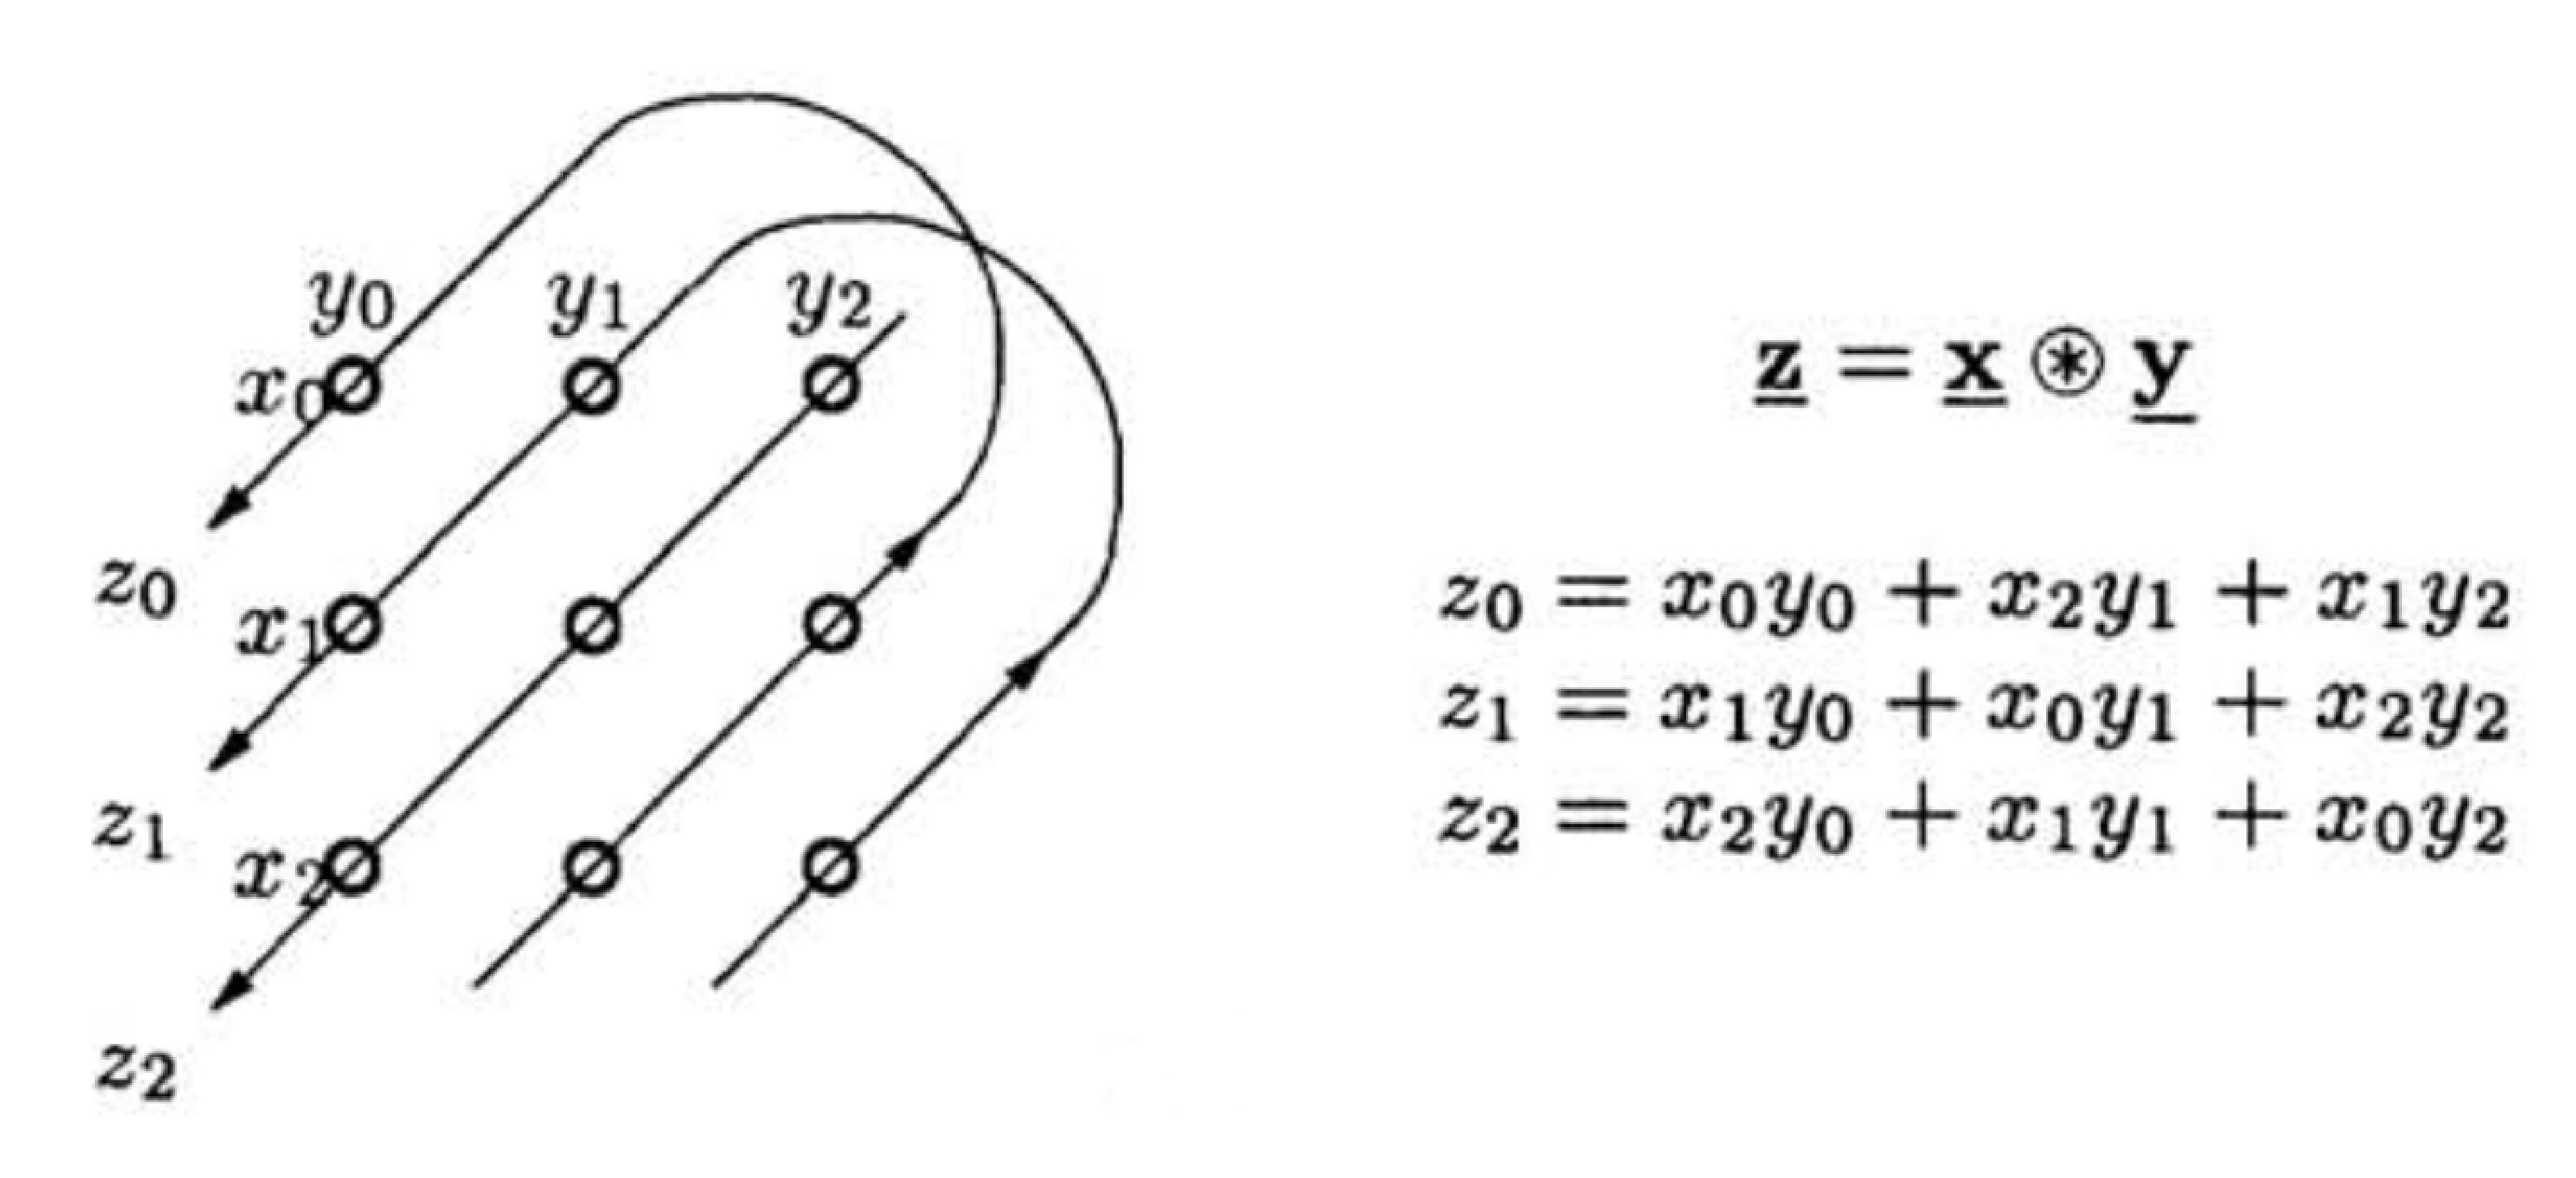
\includegraphics[width=0.85\textwidth]{imgs/circular_convolution_visualization_hor.eps}
			\caption{Visualization of circular convolution as compressed outer product for $3$-dimensional vectors. Image source \cite{Plate1994a}}
			\label{fig:circ_conv}
		\end{figure}
		The neutral element regarding circular convolution is $\pmb{1} = \left(1, 0, \cdots, 0\right)$. 
		One important property of this operation is the fact, that circular convolution can efficiently be computed using the \ac{DFT}.
		The \ac{DFT} is defined as the function
		\[
		\abb{\ac{DFT}}{\mathbb{C}^{D}}{\mathbb{C}^{D}}{x}{\left(\sum_{j=0}^{D-1} x_{j} \zeta_{D}^{-jk} \right)_{k=0}^{D-1}} \qquad \textrm{ with } \zeta_{D} = \exp\left( \frac{i 2 \pi}{D} \right).
		\]
		Similarly, the \ac{IDFT} is defined as the function 
		\[
		\abb{\ac{IDFT}}{\mathbb{C}^{D}}{\mathbb{C}^{D}}{x}{\left( \frac{1}{D} \sum_{j=0}^{D-1} x_{j} \zeta_{D}^{jk} \right)_{k=0}^{D-1}}.
		\]
		From the convolution theorem \cite[Chap. 6]{Bracewell2000} we know, that we can calculate the circular convolution of any two vectors $v, w \in V_{D}(N)$ by
		\[
		v \varoast w = \ac{IDFT}\left(\ac{DFT}(v) \odot \ac{DFT}(w) \right),
		\]
		with $\odot$ denoting element-wise multiplication in this case.
		This induces that circular convolution obeys the same rules (commutativity and associativity) as element-wise multiplication, as both operations are the same except for a change of basis. 
	\end{enumerate}
\end{ex}
As mentioned earlier, one of the most important features of (high-dimensional) \acp{VSA} is the fact that two random vectors are likely to be dissimilar.
We will derive this result in the following Theorem.
\begin{theorem}
	\label{theorem:VSA_cossim_distribution}
	Let $\left(V_{D}(N), \varoast, \oplus, \phi \right)$ a \acl{VSA}. 
	For two randomly chosen vectors $v, w \in V_{D}(N)$, the distribution of the similarity $\phi\left(v,w\right)$ is a version of the beta-distribution $\beta\left(\frac{D-1}{2},\frac{D-1}{2}\right)$ scaled and shifted to the interval $\left[-1,1\right]$ with mean $\mu=0$ and variance $\sigma^2=\frac{c^2}{D}$ up to a constant $c$. The standardized distribution trends with growing $D$ to a normal distribution.
\end{theorem}
\begin{proof}
	We will only give the proof of this Theorem for real valued \acp{VSA}, i.e. $N \subseteq \mathbb{R}$ and $\phi$ as the cosine similarity.
	Without loss of generality, we assume the vectors $v,w$ picked randomly from the unit sphere $\mathbb{S}^{D-1} = \{ v \in \mathbb{R}^{D} | \norm{v} = 1 \}$, as we can simply normalize the vectors by $\frac{v}{\norm{v}}$.
	Since binary \acp{VSA} can be associated with a euclidean sphere as well, the same result can be proven for those architectures with similar arguments (see \cite{Kanerva1988} for details).
	Due to symmetry of the unit sphere $\mathbb{S}^{D-1}$, we can furthermore - again without loss of generality - choose one vector as a unit vector, i.e. $w=\left(1, 0 , \cdots, 0\right)$.
	Thereby, the cosine similarity for $v=\left(v_{0}, \cdots, v_{D-1}\right)$ is given by $\phi\left(v,w\right) = v_{0}$
	By fixing one coordinate, we get the constraint $\sum_{i=1}^{D-1} v_{i}^{2} = 1-v_{0}^{2}$ which is equivalent to a lower dimensional sphere $\mathbb{S}^{D-2}$ with radius $\sqrt{1-v_{0}^2}$.
	Hence the cosine similarity $\phi\left(v,w\right)=:x$ is proportional to the surface of a conical frustum constructed from $\mathbb{S}^{D-2}$ with radius $\sqrt{1-x^{2}}$, slope $\frac{1}{\sqrt{1-x^{2}}}$ and some height $h$, i.e. the density function is proportional to
	\[
	f_{\phi(v,w)}(x) \propto \frac{\sqrt{1-x^{2}}^{(D-2)}}{\sqrt{1-x^{2}}} h \propto \left(1-x^{2}\right)^{\frac{D-3}{2}}.
	\]
	Substituting $x=2u-1$, we get 
	\[
	\left(1-\left(2u-1\right)^{2}\right)^{\frac{D-3}{2}} \propto \left(u-u^2\right)^{\frac{D-3}{2}} = \left(u \left(1-u\right)\right)^{\frac{D-3}{2}} = u^{\left(\frac{D-1}{2}-1\right)} \left(1-u\right)^{\left(\frac{D-1}{2}-1\right)},
	\]
	which is the density function of the beta distribution $\beta\left(\frac{D-1}{2},\frac{D-1}{2}\right)$.
	Thus, the cosine similarity is also beta distributed, but scaled and shifted to the interval $\left[-1,1\right]$ by $x=2u-1$.\\
	For $\alpha=\beta=\frac{D-1}{2}$, the mean of the beta distribution is $\tilde{\mu}=\frac{1}{2}$. Applying the substitution, we get the mean of the shifted distribution $\mu = 2\tilde{\mu }-1 = 0$.\\
	Making use of the simplification that the distribution of similarity is the same as the distribution in the first coordinate, the variance is given by the expected value of the square value of the first coordinate, i.e. $\mathbb{E}(v_{0}^{2})$.
	Since all coordinate are identically distributed, we get
	\[
	\mathbb{E}(v_{0}) = \frac{1}{D} \sum_{i=0}^{D-1} \mathbb{E}(v_{i}^2)= \frac{1}{D} \underbrace{\mathbb{E}\left(\sum_{i=0}^{D-1} v_{i}^2\right)}_{=:c^2}=\frac{c^2}{D}.
	\]
	Hence variance of the distribution of the cosine similarity is $\sigma^2=\frac{c^2}{D}$.
	In the particular case of the unit sphere $\mathbb{S}^{D-1}$, we get $c^{2}=1$ and a variance of $\sigma^2=\frac{1}{D}$.\\
	To see the convergence behaviour of the standardized distribution, we look at the logarithm of its density function %$f_{\phi(v,w)}\left(\frac{x}{\sqrt{D}}\right)$
	\begin{equation}
	\label{eq:log_dens}
	\log\left(f_{\phi(v,w)}\left(\frac{x}{\sqrt{D}}\right)\right) = \frac{D-3}{2}\log\left(1-\frac{x^2}{D}\right) + C.
	\end{equation}
	Using the Tayler series approximation of the logarithm, equation \ref{eq:log_dens} transforms to
	\begin{align*}
		\log\left(f_{\phi(v,w)}\left(\frac{x}{\sqrt{D}}\right)\right) &= \frac{D-3}{2}\left(-\frac{x^2}{D} + \frac{x^4}{4D} \pm \ldots \right) + C = -\frac{1}{2}x^2 + \frac{3}{2D}x^2 + \mathcal{O}\left(\frac{x^4}{D}\right)  + C  \\
		&\longrightarrow -\frac{1}{2}x^2 + C = \log\left(f_{\mathcal{N}}\left(x\right)\right) \textrm{ for } D \longrightarrow \infty.
	\end{align*}
	Hence, with growing $D$ the standardized distribution of the cosine similarity trends to a normal distribution. 
\end{proof} 
Theorem \ref{theorem:VSA_cossim_distribution} states, that the probability of finding two random, non-orthogonal vectors in a \ac{VSA} decreases with growing vector dimension.
\begin{figure}[t!]
	\centering
	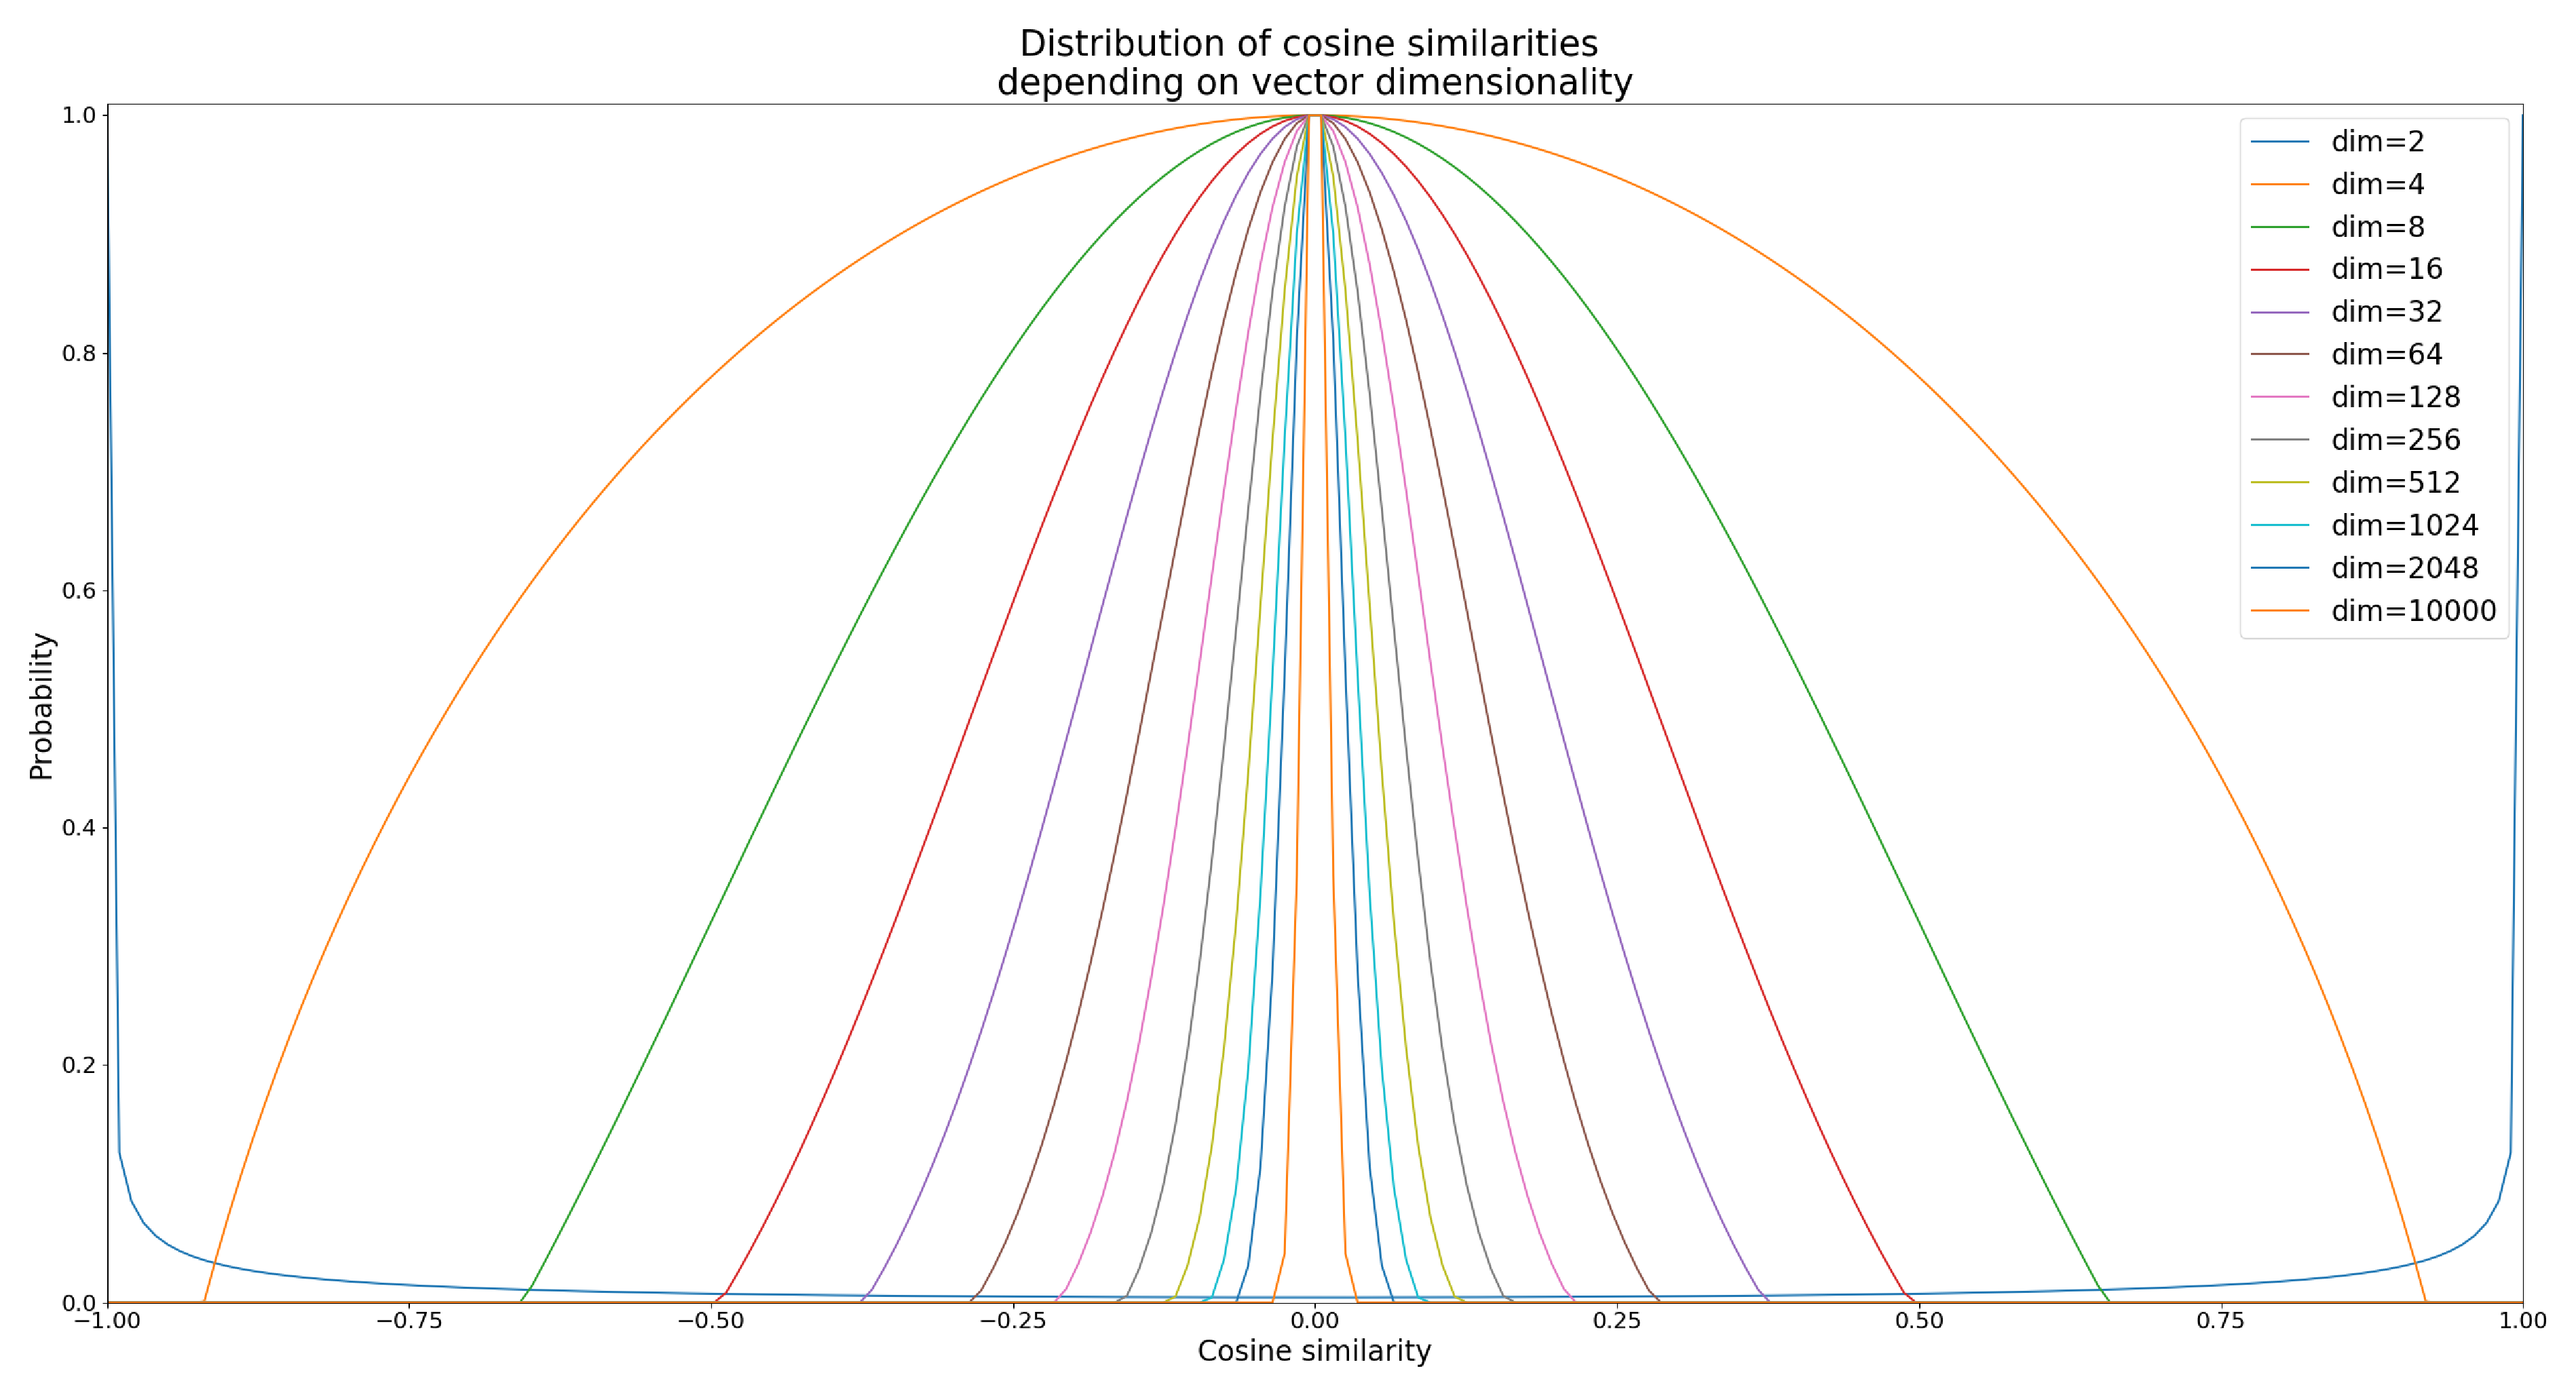
\includegraphics[width=0.85\textwidth]{imgs/distributions_cosine_sims.eps}
	\caption{Visualization of cosine similarity distributions for different vector dimensions \todo{remove figure title in python, make labels larger for better readability}}
	\label{fig:cosine_dist}
\end{figure}
Fig. \ref{fig:cosine_dist}, which shows the probability distributions of cosine similarity for different vector dimensions, illustrates this result. 
Furthermore, Theorem \ref{theorem:VSA_cossim_distribution} allows us to give a more formal definition of the term "dissimilar".
\begin{defn}
	\label{def:similar}
	Let $(V_{D}(N), \varoast, \oplus, \phi)$ be a \acrfull{VSA} of dimension $D$ and $c \in \mathbb{N}$ a constant. We call any two vectors $v, w \in V_{D}(N)$ \emph{dissimilar}, if 
	\[ 
	\left| \phi(v,w) \right| \leq \epsilon, \textrm{ with } \epsilon:=\tfrac{c}{\sqrt{D}}.
	\]
	Analogously, we call any two vectors $v, w \in V_{D}(N)$ \emph{similar}, if	$\left| \phi(v,w) \right| > \epsilon$. 
	Similar vectors are denoted by $v \approx w$. \\
	\todo{maybe use two different $\epsilon$ for $2$ or $3$ for definition of similar and highly similar?}
\end{defn}
Definition \ref{def:similar} can also be stated as follows: we consider any two vectors similar, if their similarity is higher than what we would expect from two randomly chosen vectors.
Therefore, we make use of the fact, that for growing dimension $D$, the cosine similarity follows approximately a normal distribution $\mathcal{N}\left(\mu, \sigma\right)$, with $\mu=0$ and $\sigma=\tfrac{1}{\sqrt{D}}$ and the so-called three-sigma-rule.
This rule, which follows from Chebyshev's inequality, states that the probability $\mathbb{P}\left(\mu-3\sigma \leq X \leq \mu+3\sigma \right) \geq 0.95$ for any unimodal distributed random variable $X$.
For normally distributed $X$, we even have
\begin{align*}
	\mathbb{P}\left(\mu-2\sigma \leq X \leq \mu+2\sigma \right) &\approx 0.954 \\
	\mathbb{P}\left(\mu-3\sigma \leq X \leq \mu+3\sigma \right) &\approx 0.997.
\end{align*}
Given Definition \ref{def:similar}, the probability of two randomly chosen vectors being similar is below \SI{5}{\percent} for $c=2$ and even below \SI{0.3}{\percent} for $c=3$, while the actual numerical interval $\left[-c\sigma, c\sigma\right]$ only depends on the vector dimension $D$.
For lower \ac{VSA} dimensions ($D \leq 50$), it can be beneficial to work with a weaker version of definition \ref{def:similar} using $c=2$, whereas for higher dimensions the stronger version can safely be used. \todo{wording}\\
Based on the definition of similarity, we derive criteria for "good" multiplication functions in \acp{VSA}.
\begin{defn}
	\label{def:binding}
	Let $(V_{D}(N), \varoast, \oplus, \phi)$ be a \acrfull{VSA} of dimension $D$. We call its multiplication function 
	\[\abb{\varoast}{V_{D}(N) \times V_{D}(N)}{K^{D}}{(v,w)}{\varoast(v,w) =: v\varoast w}\]
	a \emph{binding function} if 
	\begin{enumerate}
		\item for any two vectors $v, w \in V_{D}(N)$, the vector $v \varoast w$ is dissimilar to both $v$ and $w$, i.e.
		\[
		\left| \phi(v,v \varoast w) \right| \leq \epsilon \textrm{ and } \left| \phi(w,v \varoast w) \right| \leq \epsilon.
		\]
		\item for any vector $v \in V_{D}(N)$, there exists a vector $\bar{v} \in V_{D}(N)$ with $v \varoast \bar{v} \approx \mathbf{1}$. We call $\bar{v}$ a \emph{pseudo-inverse} element. 
		If furthermore $v \varoast \bar{v} = \mathbf{1}$, we call the vector $\bar{v}$ \emph{exact inverse}.
	\end{enumerate}
\end{defn}
It is worth noting, that all multiplication operations mentioned in example \ref{ex:VSAs} fulfill the criteria for binding functions as stated in Definition \ref{def:binding}. 
The first criteria is intended to allow structured representations in \acp{VSA}.
Representations built solely upon an addition function lack a mechanism to impose structure, as the sum of vectors is similar to all summands.
For continuous \acp{VSA}, this result is straightforward due to the linearity of the dot product, but it holds true for \acp{BSC} as well.
Therefore, summing vectors only allows to encode unordered sets of entities.
The property of binding functions to map two vectors to a vector dissimilar to both inputs enables structured representations.\\
The second criteria of Definition \ref{def:binding} for binding functions is the basis to decode or recover the individual vector ingredients from structured representations.
The existence of a (pseudo-) inverse element allows the retrieval of $v,w \in V_{D}(N)$ from $v \varoast w$ by
\begin{equation}
\label{eq:retrieval}
\bar{v} \varoast \left(v \varoast w\right) = \underbrace{\bar{v} \varoast v}_{\approx \mathbf{1}} \varoast w = \tilde{w} \approx w.
\end{equation}
In case of exact inverse elements, the right hand side of equation \ref{eq:retrieval} becomes an exact equality $\tilde{w}=w$.
In most cases, however, the result $\tilde{w}$ is not exactly equal to $w$, but similar.
It is this inherent inexactness of most \acp{VSA} what makes them suitable candidates for cognitive modelling \cite{Eliasmith2013}.
On the other hand, it imposes a functional demand for a clean-up memory.
A clean-up memory is a mechanism, which maps noisy versions of vectors like $\tilde{w}$ to their exact counterparts, here $w$.
Therefore, we need to have a set of vectors, which represent established concepts or symbols the system has knowledge of.

\begin{defn}
	\label{def:clean-up-mem}
	Let $(V_{D}(N), \varoast, \oplus, \phi)$ be a \acrfull{VSA} of dimension $D$ with binding function $\varoast$.
	We call a finite subset $\vartheta \subsetneq V_{D}(N)$ a \emph{vocabulary}.
	A function $\abbil{\gamma}{K^{D}}{\vartheta}$ is called a \emph{clean-up memory}, if 
	\begin{enumerate}
		\item for any vector $v\in K^{D}$ we have
		\[
		\phi\left(v, \gamma(v)\right) > \phi\left(v, w\right), \textrm{ for any vector } w \in \vartheta, \gamma(v) \neq w.
		\]
		\item for any two similar vectors $ v \neq \tilde{v} \in K^{D}, v \in \vartheta$, i.e. $\tilde{v} \approx v$, we have $\gamma(\tilde{v})=v$.
	\end{enumerate}
\end{defn}
Definition \ref{def:clean-up-mem} states, that the cleaned-up version of a vector is more similar to the original (noisy) version than any other vector in the vocabulary.

%----------------------------------------------------------------------------------------------------------
\section{The \acl{SPA}}
\label{sec:spa}
%----------------------------------------------------------------------------------------------------------

In this section, we focus on one particular \ac{VSA}, namely the \ac{SPA}, as we will be using it throughout this work.
The \ac{SPA} is an adoption of Plate's previously mentioned \acp{HRR} (cf. example \ref{ex:VSAs}).
Revisiting definition \ref{def:VSA}, the underlying number field of the \ac{SPA} is the field of real numbers, i.e. $N \subseteq \mathbb{R}$, the addition $\oplus$ resp. multiplication $\varoast$ operations are element-wise addition resp. circular convolution and the cosine similarity serves as measure of similarity $\phi$.
We will use $\mathcal{S}(D)$ as a short notation for the $D$-dimensional \ac{SPA} $(V_{D}(\mathbb{R}), \varoast, \oplus, \phi)$.
Eliasmith gives an in-depth description of the \ac{SPA} in \cite{Eliasmith2013}.
However, we recapitulate some important properties, which will be used later in this work.
\begin{figure}[t!]
	\centering
	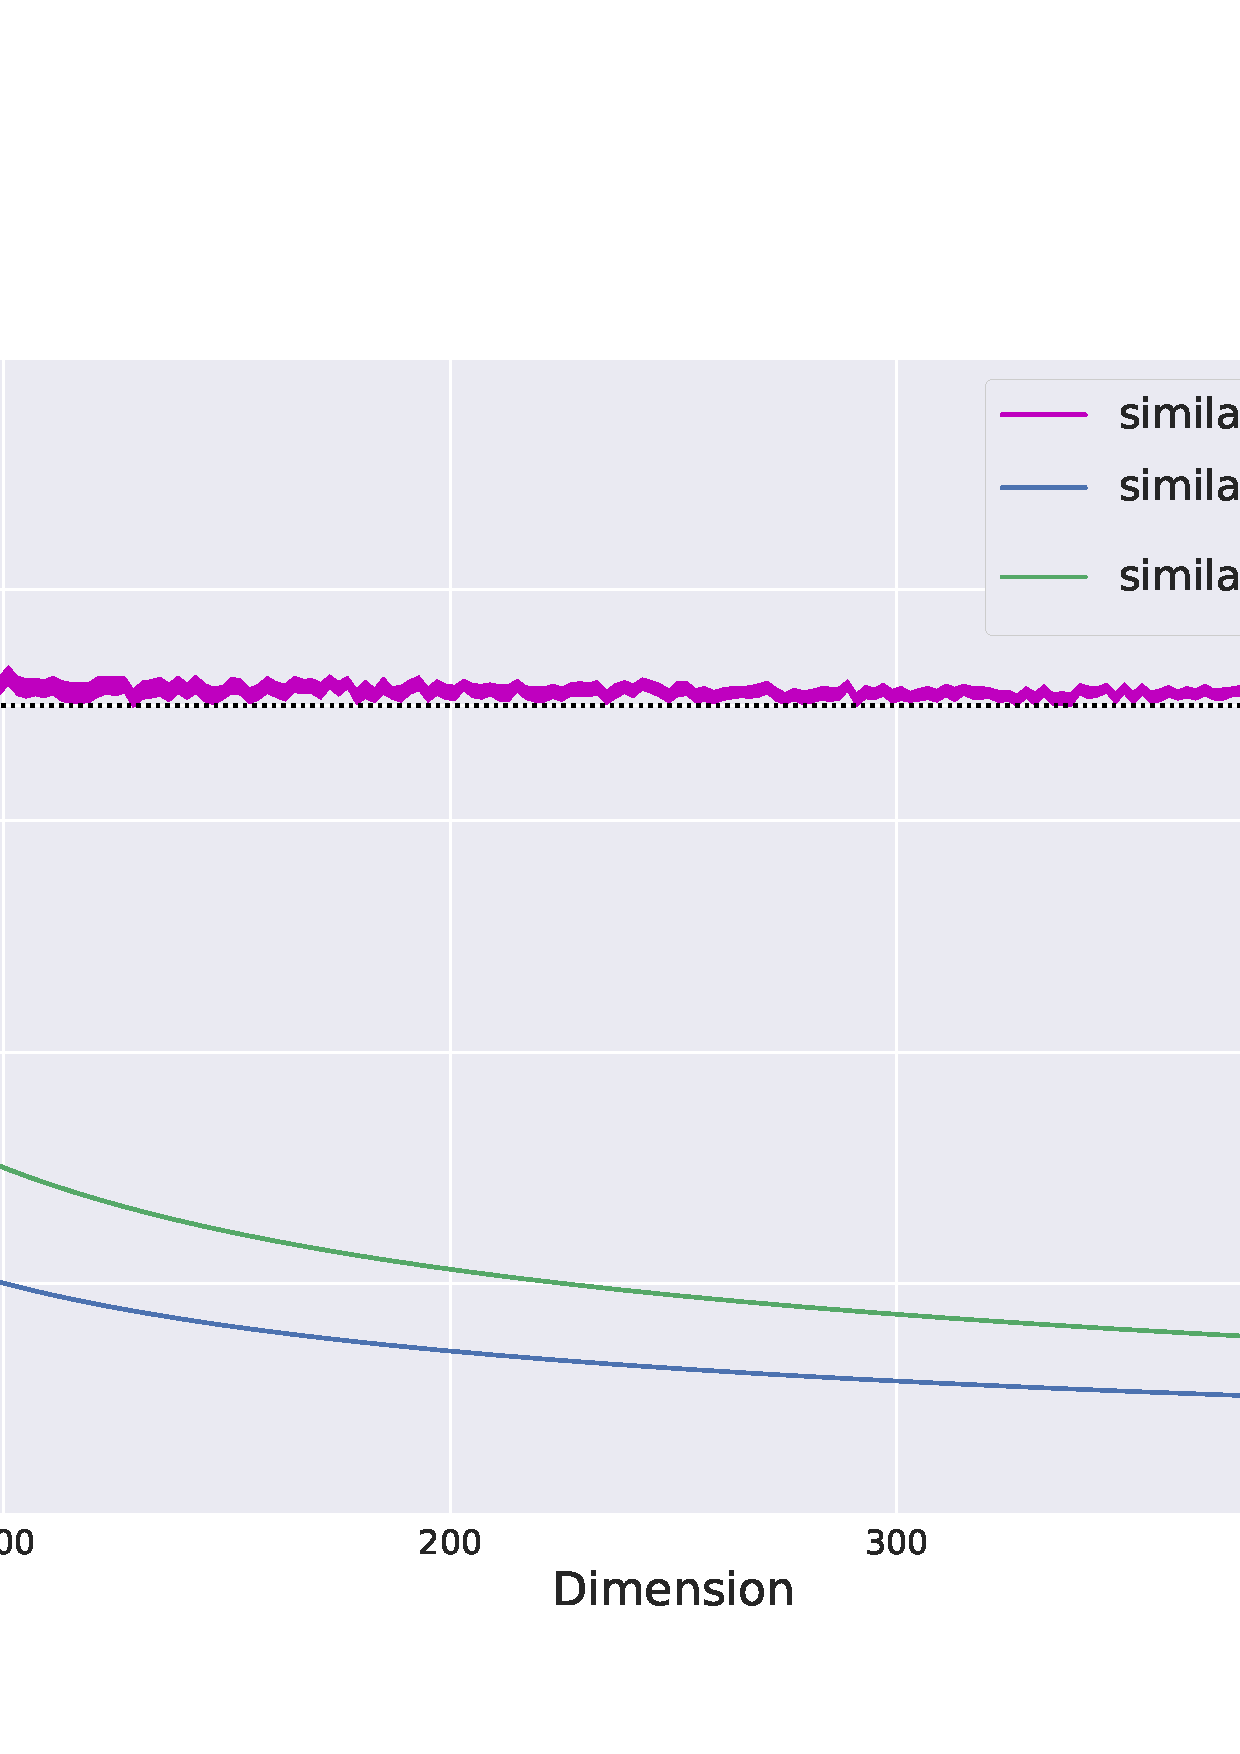
\includegraphics[width=1.0\textwidth]{imgs/pseudo_inverse_tsplot.png}
	\caption{Visualization of the similarity $\phi\left(\mathbf{1}, v \varoast \bar{v}\right)$ between the neutral element $\mathbf{1}$ and the result of applying the pseudo-inverse to different vectors for varying vector dimensions. This plot shows the result of $100$ samples compared to the similarity threshold $\epsilon$.}
	\label{fig:pseudo_inv}
\end{figure}
\begin{lemma}
	\label{lemma:spa_pseudo_inv}
	Let $v=\left(v_0, \ldots, v_{D-1}\right)$ be an element of a $D$-dimensional \ac{SPA} $\mathcal{S}(D)$, i.e. $v_0, \ldots, v_{D-1} \in \mathbb{R}$.
	The vector $\bar{v}=\left(v_0, v_{D-1}, \ldots, v_{1}\right)$ is a pseudo-inverse element of $v$ with respect to circular convolution, i.e. $v \varoast \bar{v} \approx \mathbf{1}$.
\end{lemma}
Here, we skip an explicit proof for this lemma but rather point to \cite[Section 3.1.2 and 3.1.3]{Plate1994} for a in-depth derivation.
However, we visualize the similarity $\phi\left(\mathbf{1}, v \varoast \bar{v}\right)$ between the neutral element $\mathbf{1}$ and the result of applying the pseudo-inverse $v \varoast \bar{v}$ compared to the similarity threshold $\epsilon$ (weak and strong version) in fig. \ref{fig:pseudo_inv}.
Therefore, we randomly chose $100$ sample vectors for various dimensions, convolved them with their pseudo-inverse and compared the result to the neutral element $\mathbf{1}$.
We observe, that this similarity remains almost constant slightly above $0.7$ and already for low vector dimensions ($D > 20$) way above the strong similarity threshold of $\epsilon=\frac{3}{\sqrt{D}}$.\\
Lemma \ref{lemma:spa_pseudo_inv} states that we can find a pseudo-inverse element $\bar{v}$ for any vector $v$ in a $D$-dimensional \ac{SPA} (given the dimension $D$ is sufficiently large).
Although we can also find an exact inverse element $v^{-1}$ for most vectors $v$, it is often more useful to work with pseudo-inverses instead of exact inverse elements.
We have already seen, that we can use the \acf{DFT} and \acf{IDFT} to calculate circular convolution efficiently by element-wise multiplication (this follows from the convolution theorem \cite[Chap. 6]{Bracewell2000}) in the frequency domain, i.e.
\[
	v \varoast w = \ac{IDFT}\left(\ac{DFT}(v) \odot \ac{DFT}(w) \right).
\]
Furthermore, the \ac{DFT} of the convolutive neutral element $\mathbf{1} = \left(1, 0, \ldots, 0\right)$ is 
\begin{equation}
	\ac{DFT}(\mathbf{1}) = \left(\exp\left(i0\right), \ldots, \exp\left(i0\right)\right) = \left(1, 1, \ldots, 1\right).
\end{equation}
This gives us a way of finding an exact inverse element $v^{-1}$ by 
\begin{equation}
	\ac{DFT}(\mathbf{1}) = \ac{DFT}(v) \odot \ac{DFT}(v^{-1}).
\end{equation}
By denoting the $j$-th element of the Fourier Vector $\ac{DFT}(v)$ with $\ac{DFT}_{j}(v)$, we get 
\begin{equation}
\label{eq:inv_elemtwise_fourier}
	\ac{DFT}_{j}(v) \odot \ac{DFT}_{j}(v^{-1}) = 1 \quad \textrm{ for } j \in \left\{0, \ldots, D-1\right\}.
\end{equation}
If we express $\ac{DFT}_{j}(v) \in \mathbb{C}$ in polar coordinates, i.e. $\ac{DFT}_{j}(v) = r_j \exp\left(i\varphi_j\right)$, we directly get from equation \ref{eq:inv_elemtwise_fourier} that $\ac{DFT}_{j}(v^{-1}) = \frac{1}{r_j} \exp\left(-i\varphi_j\right)$.
By using the symmetry property of the real-valued \ac{DFT}, we can see that the transform $\ac{DFT}_j(\bar{v})$ of the pseudo-inverse element $\bar{v}$ from Lemma \ref{lemma:spa_pseudo_inv} is the complex conjugate of $\ac{DFT}_j(v)$, i.e. we can write $\ac{DFT}_j(\bar{v}) = r_j \exp\left(-i\varphi\right)$ in polar coordinates.
From those equations, we can see that the pseudo-inverse $\bar{v}$ has the same norm as the original vector $v$, i.e. $\norm{v} = \norm{\bar{v}}$, whereas the norm of the exact inverse $v^{-1}$ can become significantly larger than the norm of $v$ in some cases.
This is due to the fact, that elements of the transform of the pseudo-inverse have the same lengths $r_j$ as the original vector, whereas the transformed elements of the exact inverse have lengths $\frac{1}{r_j}$, which can become significantly large when $r_j$ is close to $0$.
The relation between the vector norm and the magnitudes in the frequency domain is given by Parseval's theorem (also known as Rayleigh's theorem) \cite[Chap. 6]{Bracewell2000}, which states
\[
\norm{v}^2 = \sum_{k=0}^{D-1} \left| v_{k} \right|^{2} = \frac{1}{D} \sum_{k=0}^{D-1} \left|\ac{DFT}_{k}\left(v\right)\right|^{2} = \sum_{k=0}^{D-1} r_{k}^{2}.
\]
This can lead to additional noise when retrieving vectors from structured representations (cf. equation \ref{eq:retrieval}).
However, there is a certain class of vectors, for which the pseudo- and exact inverse element coincide.
\begin{defn}
	\label{def:unitary_vec}
	Let $v$ be a vector in a $D$-dimensional \ac{SPA} $\mathcal{S}(D)$ with exact and pseudo-inverse elements $v^{-1}$ and $\bar{v}$ respectively.
	We call $v$ a \emph{unitary vector}, if and only if $v^{-1} = \bar{v}$. 
	We denote the set of unitary vectors by $\mathcal{U} \subset \mathcal{S}(D)$.
\end{defn}
\begin{defn}
	\label{def:conv_power}
	Let $v$ be a vector in a $D$-dimensional \ac{SPA} $\mathcal{S}(D)$. We define the \emph{convolutive power} by an exponent $p \in \mathbb{R}$ by
	\[
	v^{p} := \Re\left(\ac{IDFT} \left(\left(\ac{DFT}_{j}\left(v\right)^{p}\right)_{j=0}^{D-1}\right)\right),
	\]
	where $\Re$ denotes the real part $a$ of a complex number $a + ib \in \mathbb{C}$.
\end{defn}
Unitary vectors take a special role in the \ac{SPA} as they have some interesting and useful properties.
\begin{lemma}
	\label{lemma:unitary_vec}
	Let $\mathcal{U}$ be the set of unitary vectors in the $D$-dimensional \ac{SPA} $\mathcal{S}(D)$. The following statements hold
 	\begin{enumerate}[label=\roman*]
		\item All elements of $\mathcal{U}$ have unit length, i.e. we have $\norm{u} = 1$ for any vector $u \in \mathcal{U}$.
		\item $\mathcal{U}$ is closed under convolutive exponentiation, i.e. $u^{p} \in \mathcal{U}$ for any $u \in \mathcal{U}$ and $p \in \mathbb{R}$.
		\item Convolution with unitary vectors preserves the norm, i.e. $\norm{v} = \norm{v \varoast u}$ for any $v \in \mathcal{S}(D), u \in \mathcal{U}$.
	\end{enumerate}
\end{lemma}
\begin{proof}
	To show, that unitary vectors have unit length, we directly calculate the first component of convolution $z :=u \varoast \bar{u}$ between a unitary vector $u$ and its pseudo-inverse $\bar{u}$:
	\[
	z_{0} = \sum_{k=0}^{D-1} u_{k} \bar{u}_{-k \Mod{D}} = \sum_{k=0}^{D-1} u_{k}^{2} = \norm{u}^{2}.
	\]
	As $u$ is a unitary vector, we have $u^{-1} = \bar{u}$ and therefore $u\varoast \bar{u} = \mathbf{1}$.
	Thus, we have for the first component of $z :=u \varoast \bar{u}$
	\[
	1 = z_{0} = \norm{u}^{2},
	\]
	which gives the first result of the lemma.\\
	To show that the set of unitary vectors $\mathcal{U}$ is closed under convolutive exponentiation, we write each component of $\ac{DFT}(u)$ for $u \in \mathcal{U}$ in polar coordinates, i.e. $\ac{DFT}_j(u) = r_j\exp\left(\varphi_j\right)$.
	From previous considerations we know that $\ac{DFT}_j(u^{-1}) = \frac{1}{r_j}\exp\left(-\varphi_j\right)$ and $\ac{DFT}_j(\bar{u}) = r_j\exp\left(-\varphi_j\right)$, which gives $r_j=1$ for $j=0, \ldots, D-1$ because $u$ is a unitary vector.
	Thus, we have for any $p \in \mathbb{R}$
	\[
	\ac{DFT}_j\left(u^{p}\right) = \ac{DFT}_j\left(u\right)^{p} = r_j^{p}\exp\left(ip\varphi\right) = 1^{p} \cdot \exp\left(ip\varphi\right),
	\]
	which makes $u^{p}$ itself a unitary vector, as all magnitudes are $1$.	\\
	To proof that convolution with unitary vectors preserves the norm, we use Parseval's theorem again. 
	For any vector $v \in \mathcal{S}(d)$ and  a unitary vector $u \in \mathcal{U}$, we denote $z:= v \varoast u$ and get 
	\begin{equation}
	\label{eq:norm_parseval}
	\norm{v \varoast u}^{2} = \sum_{k=0}^{D-1} \left|z_{k}\right|^{2} = \frac{1}{D} \sum_{k=0}^{D-1} \left|\ac{DFT}_{k}(z)\right|^{2} = \frac{1}{D} \sum_{k=0}^{D-1} \left|\ac{DFT}_{k}(v) \cdot \ac{DFT}_{k}(u)\right|^{2}.
	\end{equation}
	Writing $\ac{DFT}_{k}(v) = r_{vk}\exp\left(i\varphi_{vk}\right)$ and $\ac{DFT}_{k}(u) = r_{uk}\exp\left(i\varphi_{uk}\right)$ in polar coordinates with $r_{uk} = 1$ for $k=0, \ldots, D-1$ as $u$ is unitary, equation \ref{eq:norm_parseval} transforms to
	\begin{equation*}
	\norm{v \varoast u}^{2} = \frac{1}{D} \sum_{k=0}^{D-1} \left|r_{vk} \exp\left(i\left(\varphi_{vk} + \varphi_{uk}\right)\right)\right|^{2} = \frac{1}{D} \sum_{k=0}^{D-1} \left|r_{vk}\right|^{2} = \frac{1}{D} \sum_{k=0}^{D-1} \left|\ac{DFT}_k\left(v\right)\right|^{2} = \norm{v}^{2}.
	\end{equation*}
\end{proof}

%----------------------------------------------------------------------------------------------------------
\section{The \acl{NEF}}
\label{sec:neural_eng}
%----------------------------------------------------------------------------------------------------------

In this section, we make a short excursion and give a brief overview of the \acf{NEF}, as we will be making use of it in forthcoming chapters.
The \ac{NEF} \cite{Eliasmith2003} is a mathematical theory, which provides a set of methods to construct biologically plausible, large-scale neural models.
These methods can be divided into the three main principles of the \ac{NEF}: \emph{representation}, \emph{transformation} and \emph{dynamics}.
The \ac{Nengo} \cite{Bekolay2014, Nengo} software suite is a python library, which implements the \ac{NEF}'s principles.
\ac{Nengo} has been used to build a variety of neural models, e.g. models of the basal ganglia system \cite{Stewart2010, Stewart2012} and \acf{Spaun} \cite{Eliasmith2012}, a large-scale, functional model of the brain, which is able to perform eight cognitive tasks.
Furthermore, \ac{Nengo} has been used to interface neural models with physical, neuromorphic hardware systems and robots \cite{Conradt2014, Stewart2016, Mirus2018a}.
Here, we give a brief introduction to the \ac{NEF}'s principles and refer to \cite{Eliasmith2003, Eliasmith2013, Bekolay2014} for more details.
\subsection{Representation}
\label{subsec:nef_representation}
The first principle of the \ac{NEF}, representation, provides mathematical tools to encode information, namely time-varying real-valued vectors, in the activity of neural populations.
It is based on the assumption, that neurons have a "preferred direction vector" in the represented space, each neuron responds most strongly to.
This assumption is grounded by the findings of \cite{Georgopoulos1989} that each neuron in motor cortex of rhesus monkeys has a different preferred arm direction.
The \ac{NEF} expands this idea to neural representations in general.
\begin{figure}[t!]
	\centering
	\subfloat[Tuning curves \label{subfig:nef_rep_tuning_curves}]{%
		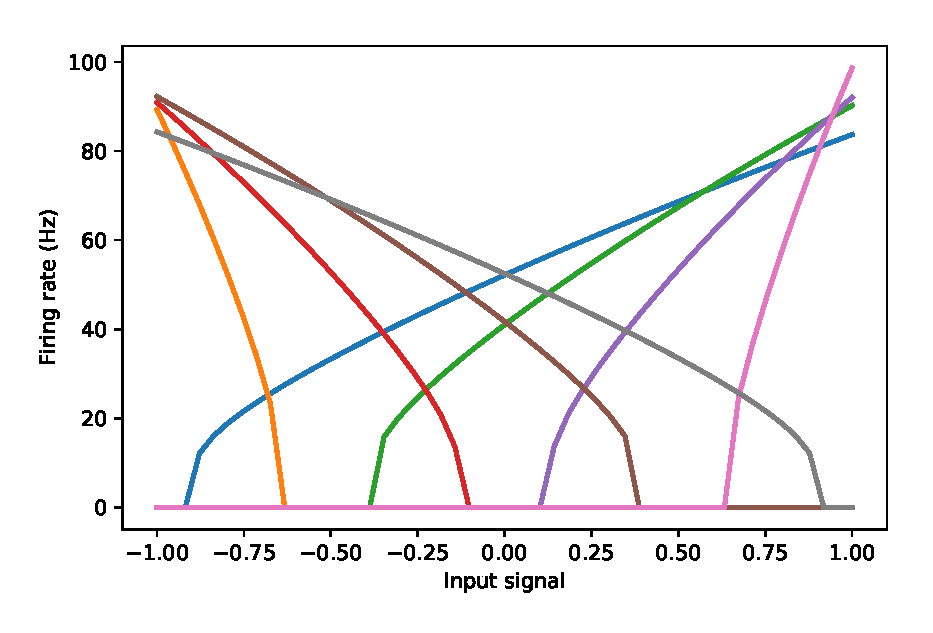
\includegraphics[width=0.45\textwidth]{imgs/NEF_tuning_curves.eps}
	}
	\subfloat[Spike times\label{subfig:nef_rep_spike_raster}]{%
		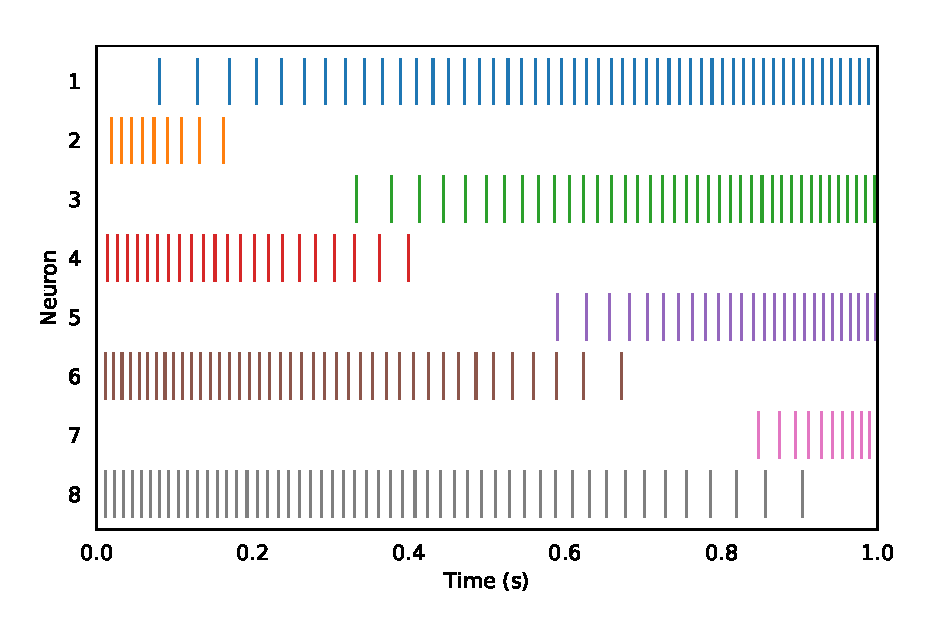
\includegraphics[width=0.45\textwidth]{imgs/NEF_spikes_raster.eps}
	}\\
	\vspace{-0.4cm}
	\subfloat[Decoded output\label{subfig:nef_rep_decoded}]{%
		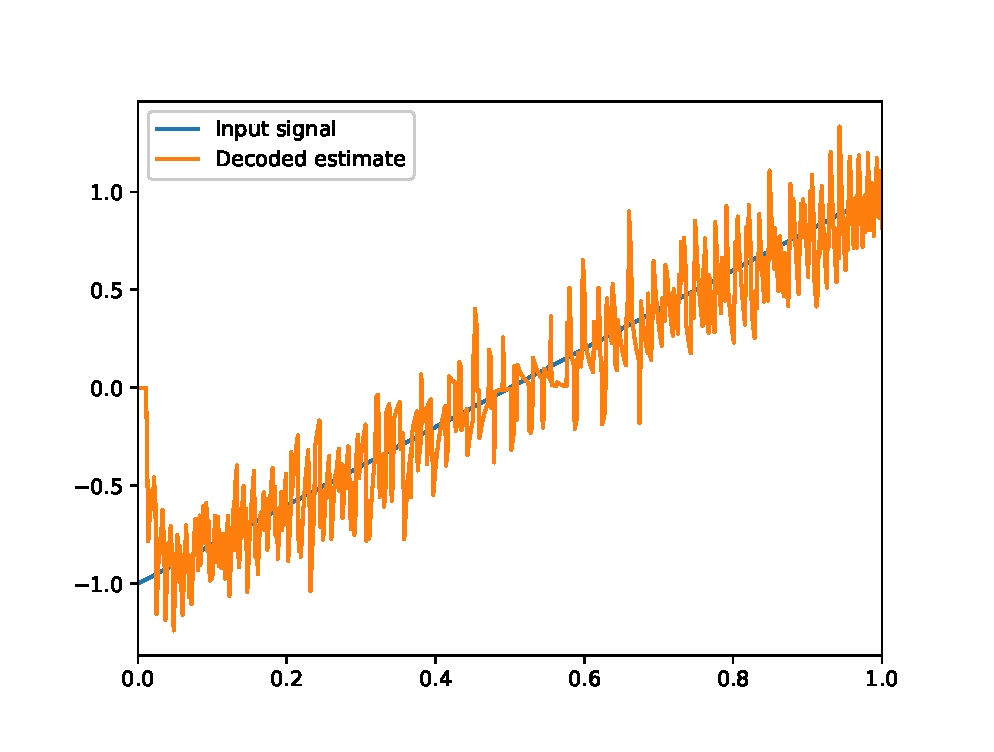
\includegraphics[width=0.45\textwidth]{imgs/NEF_decoded_output.eps}
	}
	\subfloat[Filtered neural activity\label{subfig:nef_rep_spike_filtered}]{%
		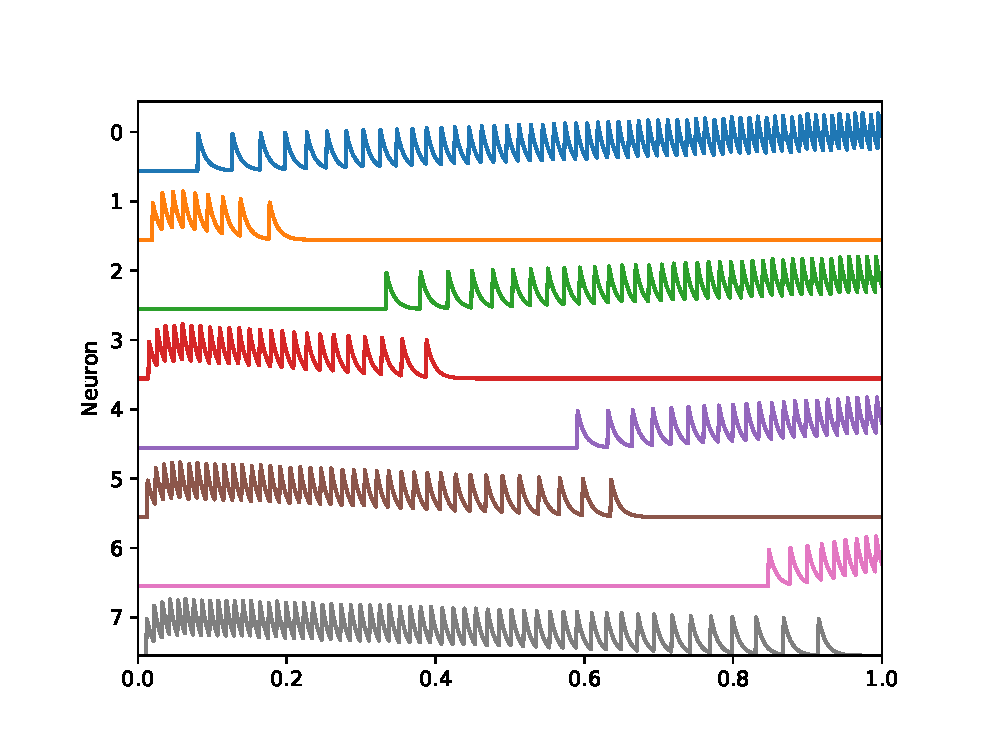
\includegraphics[width=0.45\textwidth]{imgs/NEF_spikes_filtered.eps}
	}
	\caption{The representation principle of the \ac{NEF}. Images adapted from \cite{Bekolay2014}}\label{fig:nef_representation}
\end{figure}
Let $A$ be a population of $N \in \mathbb{N}$ neurons encoding a subset $V$ of a real-valued vector space, i.e. $V\subseteq \mathbb{R}^{n}$.
Given a function $\abbil{\mathbf{x}}{\mathbb{R}}{V}$, we can write the activity $a_{i}$ of the $i$-th neuron in a neural population encoding a time-varying vector $\mathbf{x}(t)$ as a spike train, i.e. a sum of delta functions
\begin{equation}
a_{i}\left(\mathbf{x}(t)\right) = \sum_{j=1}^{m_{i}} \delta(t - t_{j}) = G_{i}(\underbrace{\alpha_{i}\langle\mathbf{e}_{i},\mathbf{x}(t)\rangle + J_{i}}_{=:c}) \quad \textrm{ for } 1 \leq i \leq N, 
\label{eq:nef_encoding}
\end{equation}
where $G_{i}$ is the spiking neural non-linearity, $\alpha_{i}$ is the gain of the neuron, $\mathbf{e}_{i}$ is the neuron's preferred direction or encoding vector and $J_{i}$ is a bias current to account for neural background activity and $t_{j}$ are the $m_{i}$ spike-times of the $i$-th neuron.
Notably, the current flowing into the cell is completely determined by $c$, whereas the spiking behaviour of the neuron model is represented by the non-linear function $G_{i}$.
The input current $c$ and therefore the \ac{NEF}'s encoding process is independent of particular spiking neuron models.\\
To decode the input values $\mathbf{x}(t)$ back out of the neural population $A$, the spike train is convolved with an exponentially decaying filter $\abbil{h}{\mathbb{R}}{\mathbb{R}}$ to simulate the process of neurons generating postsynaptic current after spiking (cf. fig. \ref{subfig:nef_rep_spike_filtered}) resulting in
\begin{equation}
\tilde{a}_{i}\left(\mathbf{x}(t)\right) = \sum_{j=1}^{m_{i}} h(t) \ast \delta(t - t_{j}) = \sum_{j=1}^{m_{i}} h(t - t_{j}).
\label{eq:nef_filtered_activity}
\end{equation}
A simple model of an exponential decaying filter is the function $\abb{h}{\mathbb{R}}{\mathbb{R}}{t}{e^{\sfrac{-t}{\tau_{p}}}}$, where $\tau_{P}$ denotes the postsynaptic time constant.
We obtain an estimation $\mathbf{\hat{x}}(t)$ of the original input $\mathbf{x}(t)$ as a weighted sum with some decoder values $\mathbf{d}_{i}$
\begin{equation}
\mathbf{\hat{x}}(t) = \sum_{i=1}^{N} \tilde{a}_{i}\left(\mathbf{x}(t)\right) \mathbf{d}_{i}.
\label{eq:nef_decoding} 
\end{equation} 
To calculate the optimal decoders $\mathbf{d}_{i}$, we need to minimize the error between input $\mathbf{x}(t)$ and decoded output $\mathbf{\hat{x}}(t)$
\begin{equation}
E = \int \left( \mathbf{x}(t) - \sum_{i=1}^{N} \tilde{a}_{i}\left(\mathbf{x}(t)\right) \mathbf{d}_{i}\right)^{2} \diff \mathbf{x}(t).
\label{eq:decoder_calculation}
\end{equation}
\ac{Nengo} solves for the decoders $\mathbf{d}_{i}$ by default using least squares optimization \cite{Eliasmith2013}[Appendix B1].
Fig. \ref{fig:nef_representation} visualizes this encoding process for $V = \left[ -1, 1\right] \subset \mathbb{R}$ and a population of $8$ neurons.
Fig. \ref{subfig:nef_rep_tuning_curves} shows the tuning curves of individual neurons, which define how these neurons respond to specific input values.
Equation \ref{eq:nef_encoding} is depicted in fig. \ref{subfig:nef_rep_spike_raster}, which shows a raster plot of the neurons' spike times based on the input signal shown in fig. \ref{subfig:nef_rep_decoded}.
Fig. \ref{subfig:nef_rep_spike_filtered}, which shows the filtered neural activity for each neuron, visualizes equation \ref{eq:nef_filtered_activity}.
Finally, fig. \ref{subfig:nef_rep_decoded} depicts the original input value as well as the estimated output of the neural populations' activity (cf. equation \ref{eq:nef_decoding}).
Note, that the neural population's decoded output is only a noisy approximation of the original input value, whose accuracy can be improved by increasing the number of neurons in the population.
\subsection{Transformation}
\begin{figure}[t]
	\centering
	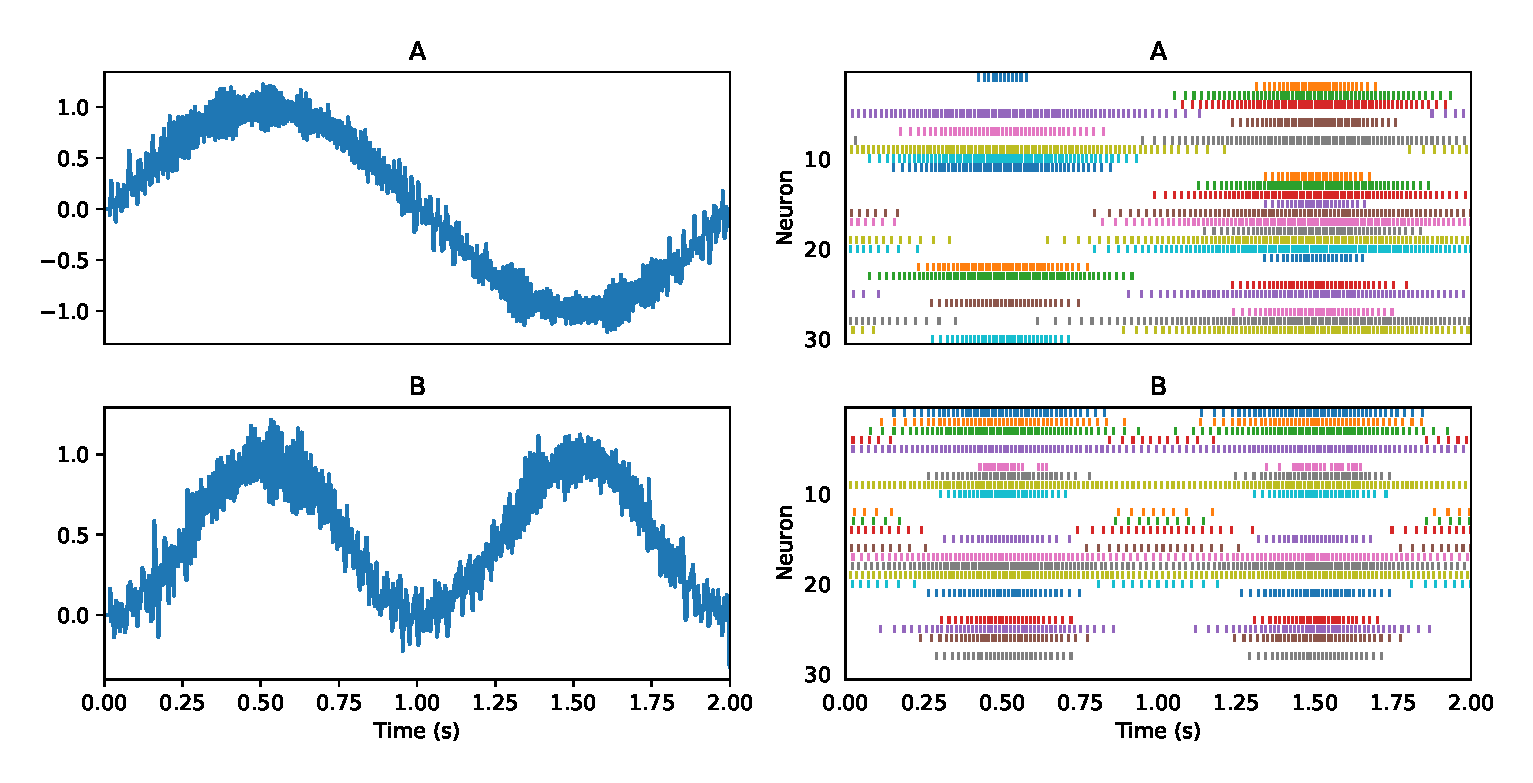
\includegraphics[width=0.85\textwidth]{imgs/NEF_transformation.eps}
	\caption{The transformation principle of the \ac{NEF}.}
	\label{fig:nef_transformation}
\end{figure}
The second main principle of the \ac{NEF}, \emph{transformation}, provides the mathematical tools to compute functions across conncetions between populations of neurons.
Let $A$ resp. $B$ be populations of $N$ resp. $M$ neurons encoding a time-varying vector $\mathbf{x}(t) \in V \subset \mathbb{R}^{n}$ resp. $\mathbf{y}(t) \in W \subset \mathbb{R}^{m}$ according to the representation principle and a function $\abbil{f}{V}{W \subset \mathbb{R}^{m}}$.
In order to approximate the funtion $f$ across a connection from population $A$ to population $B$, we use the tools of the representation principle, but we calculate a different set of decoder values $\mathbf{d}_{i}^{f}$ for population $A$ by minimizing the error
\begin{equation}
\label{eq:nef_transformation}
E = \int \left( f(\mathbf{x}(t)) - \sum_{i=1}^{N} \tilde{a}_{i}\left(\mathbf{x}(t)\right) \mathbf{d}_{i}^{f}\right)^{2} \diff \mathbf{x}(t).
\end{equation}
Given encoders $\mathbf{e}_{j}^{B}$ and gain $\alpha_{j}^{B}$ for $1 \leq j \leq M$ of population $B$, we can derive a weight matrix for the connection from $A$ to $B$ approximating the function $f$ by
\begin{equation}
w_{ij} = \alpha_{j}^{B} \mathbf{d}_{i}^{f} L \mathbf{e}_{j}^{B} \quad \textrm{for } 1 \leq i \leq N \textrm{ and } 1 \leq j \leq M, 
\end{equation}
where $L$ is a $M \times N$ linear operator. 
Here, the \ac{NEF} makes the assumption, that connection weights can be factored into encoders, decoders and a linear transform.
Fig. \ref{fig:nef_transformation} visualizes this \ac{NEF}'s transformation principle for $V = W = \left[ -1, 1\right] \subset \mathbb{R}$, two neural populations $A$, $B$ containing $30$ neurons each.
The left resp. right panel of plots shows the populations' decoded outputs resp. the neurons' spike times.
Population $A$ uses the representation principle to encode a sine function, whereas the transformation principle was used to calculate the function $\abb{f}{V}{W}{x}{f(x)=x^{2}}$ across the connection from $A$ to $B$.

\subsection{Dynamics}
\begin{figure}[t]
	\centering
	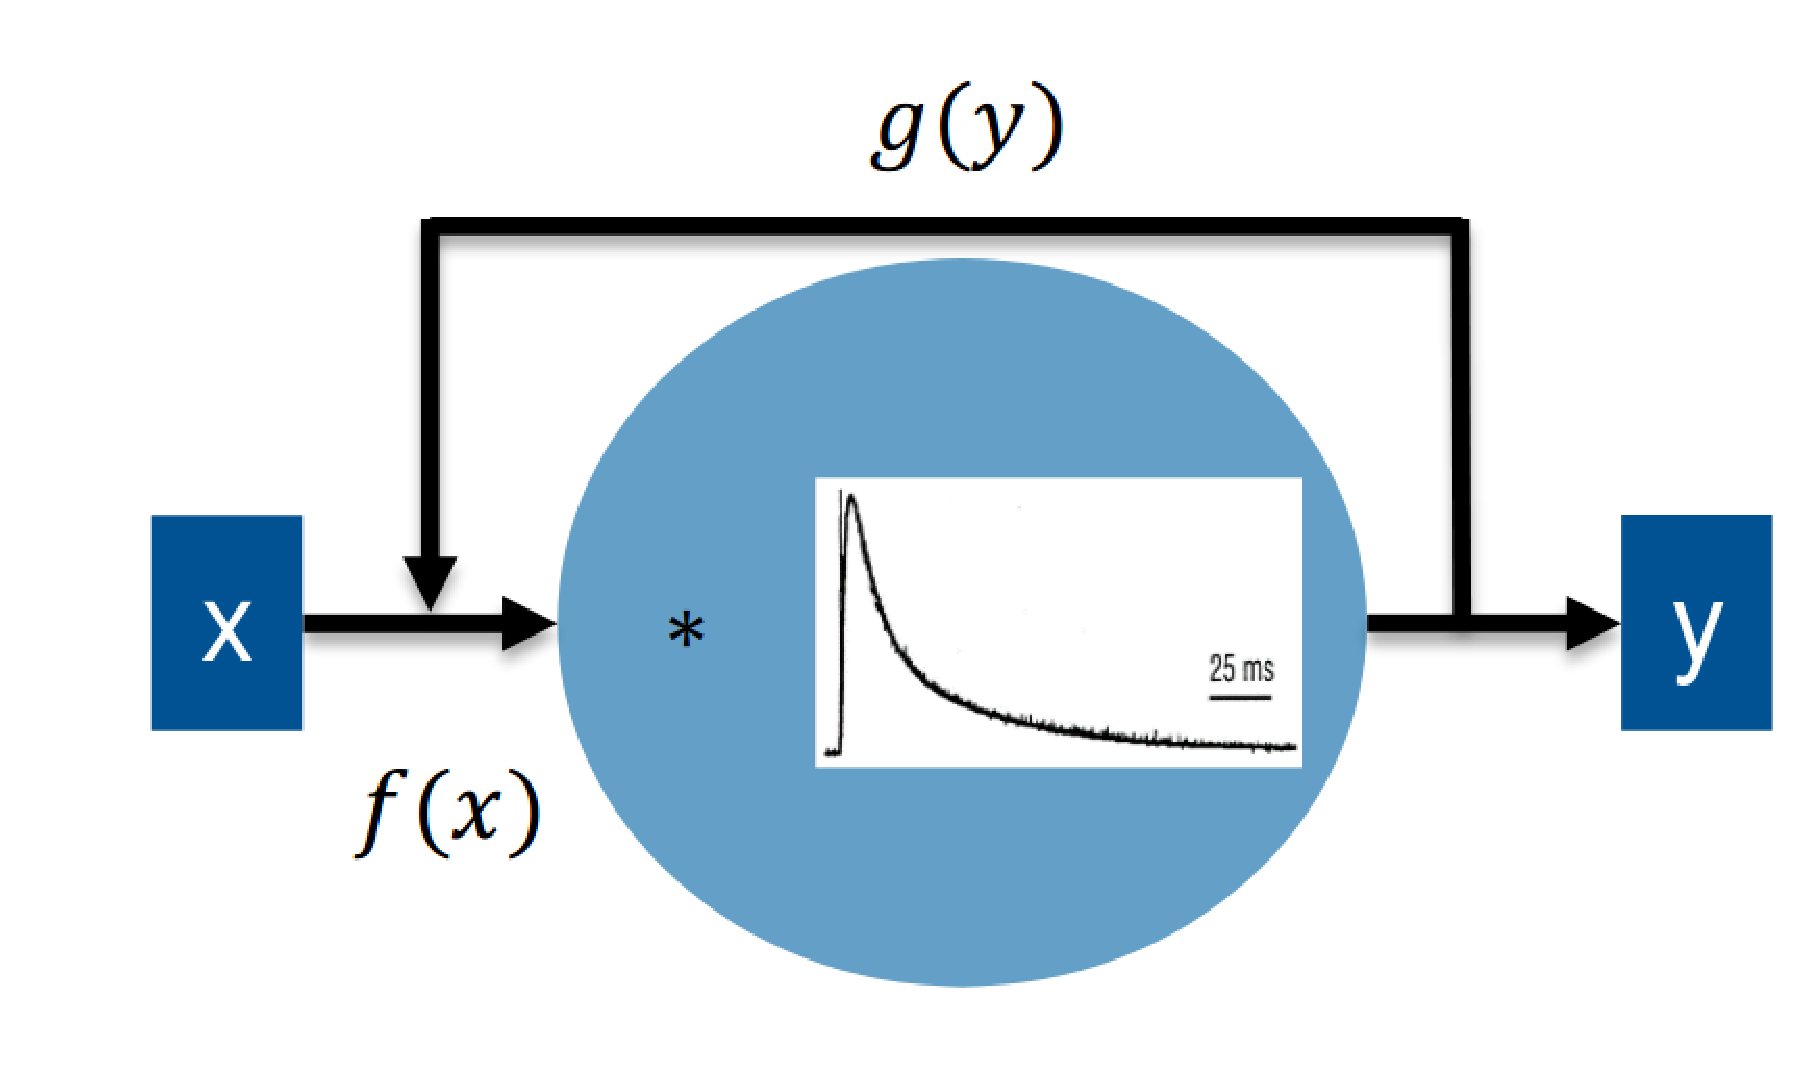
\includegraphics[width=0.85\textwidth]{imgs/NEF_recurrent.eps}
	\caption{The dynamics principle of the \ac{NEF} for recurrent connections. \todo{make a better figure!}}
	\label{fig:nef_dynamics}
\end{figure}
The third main principle of the \ac{NEF}, \emph{dynamics}, provides a set of mathematical tools to implement dynamical systems in neural populations through recurrent connections.
Let $A$ be a population of neurons with an incoming connection approximating the function $\abbil{f}{V}{W \subset \mathbb{R}^{m}}$ and a recurrent connection approximating the function $\abbil{g}{W}{W}$ (cf. fig. \ref{fig:nef_dynamics}).
Thus, the overall function the population is approximating is 
\begin{equation}
\mathbf{y}(t) = h(t) \ast \left(f(\mathbf{x}(t)) + g(\mathbf{y}(t))\right)
\label{eq:nef_dyn}
\end{equation}
with exponential decaying filter function $\abb{h}{\mathbb{R}}{\mathbb{R}}{t}{e^{\sfrac{-t}{\tau}}}$.
By applying the Laplace transform to equation \ref{eq:nef_dyn}, we get
\begin{equation}
\label{eq:nef_dyn_laplace}
\mathbf{Y}(s) = \frac{1}{1 + s\tau}\left(F(\mathbf{X}(s)) + G(\mathbf{Y}(s))\right).
\end{equation}
We can rearrange equation \ref{eq:nef_dyn_laplace} to
\begin{equation}
s\mathbf{Y}(s) = \frac{G(\mathbf{Y}(s))-\mathbf{Y}(s)}{\tau} + \frac{F(\mathbf{X}(s))}{\tau}.
\end{equation}
Transforming back leads to the differential equation
\begin{equation}
\frac{\partial \mathbf{y}(t)}{\partial t} = \frac{g(\mathbf{y}(t)-y)}{\tau} + \frac{f(\mathbf{x}(t))}{\tau}.
\end{equation}
Thus, to construct a neural model approximating a differential equation of the form 
\begin{equation}
\frac{\mathbf{y}(t)}{\partial t} = a(\mathbf{y}(t)) + b(\mathbf{x}(t))
\label{eq:nef_dyn_diffeq}
\end{equation}
with functions $\abbil{a}{W}{W}$ and $\abbil{b}{V}{W}$, the first two principles of the \ac{NEF} can be used to create a neural population of the form as shown in fig. \ref{fig:nef_dynamics}.
By setting the functions $g(\mathbf{y}(t))=\tau a(\mathbf{y}(t)) + \mathbf{y}(t)$ and $f(\mathbf{x}(t))=\tau b(\mathbf{x}(t))$, we obtain a neural model approximating the desired dynamical system described by the differential equation \ref{eq:nef_dyn_diffeq}.


\section{Cognitive Modelling with \aclp{VSA}}
In this section, we give a brief introduction of how we can use the theory of in \ref{sec:math_prop_vsas} and to \ref{sec:spa} to represent (structured) information using \acp{VSA}.
We give a general overview of different ways to establish vocabularies containing atomic vectors and how we can build more complex representations from those elementary ingredients.
Furthermore, we will see how these representations can be implemented in \acp{SNN} using the principles of the \ac{NEF} described in \ref{sec:neural_eng}.
\subsection{Vocabularies}
\begin{figure}[t]
	\centering
	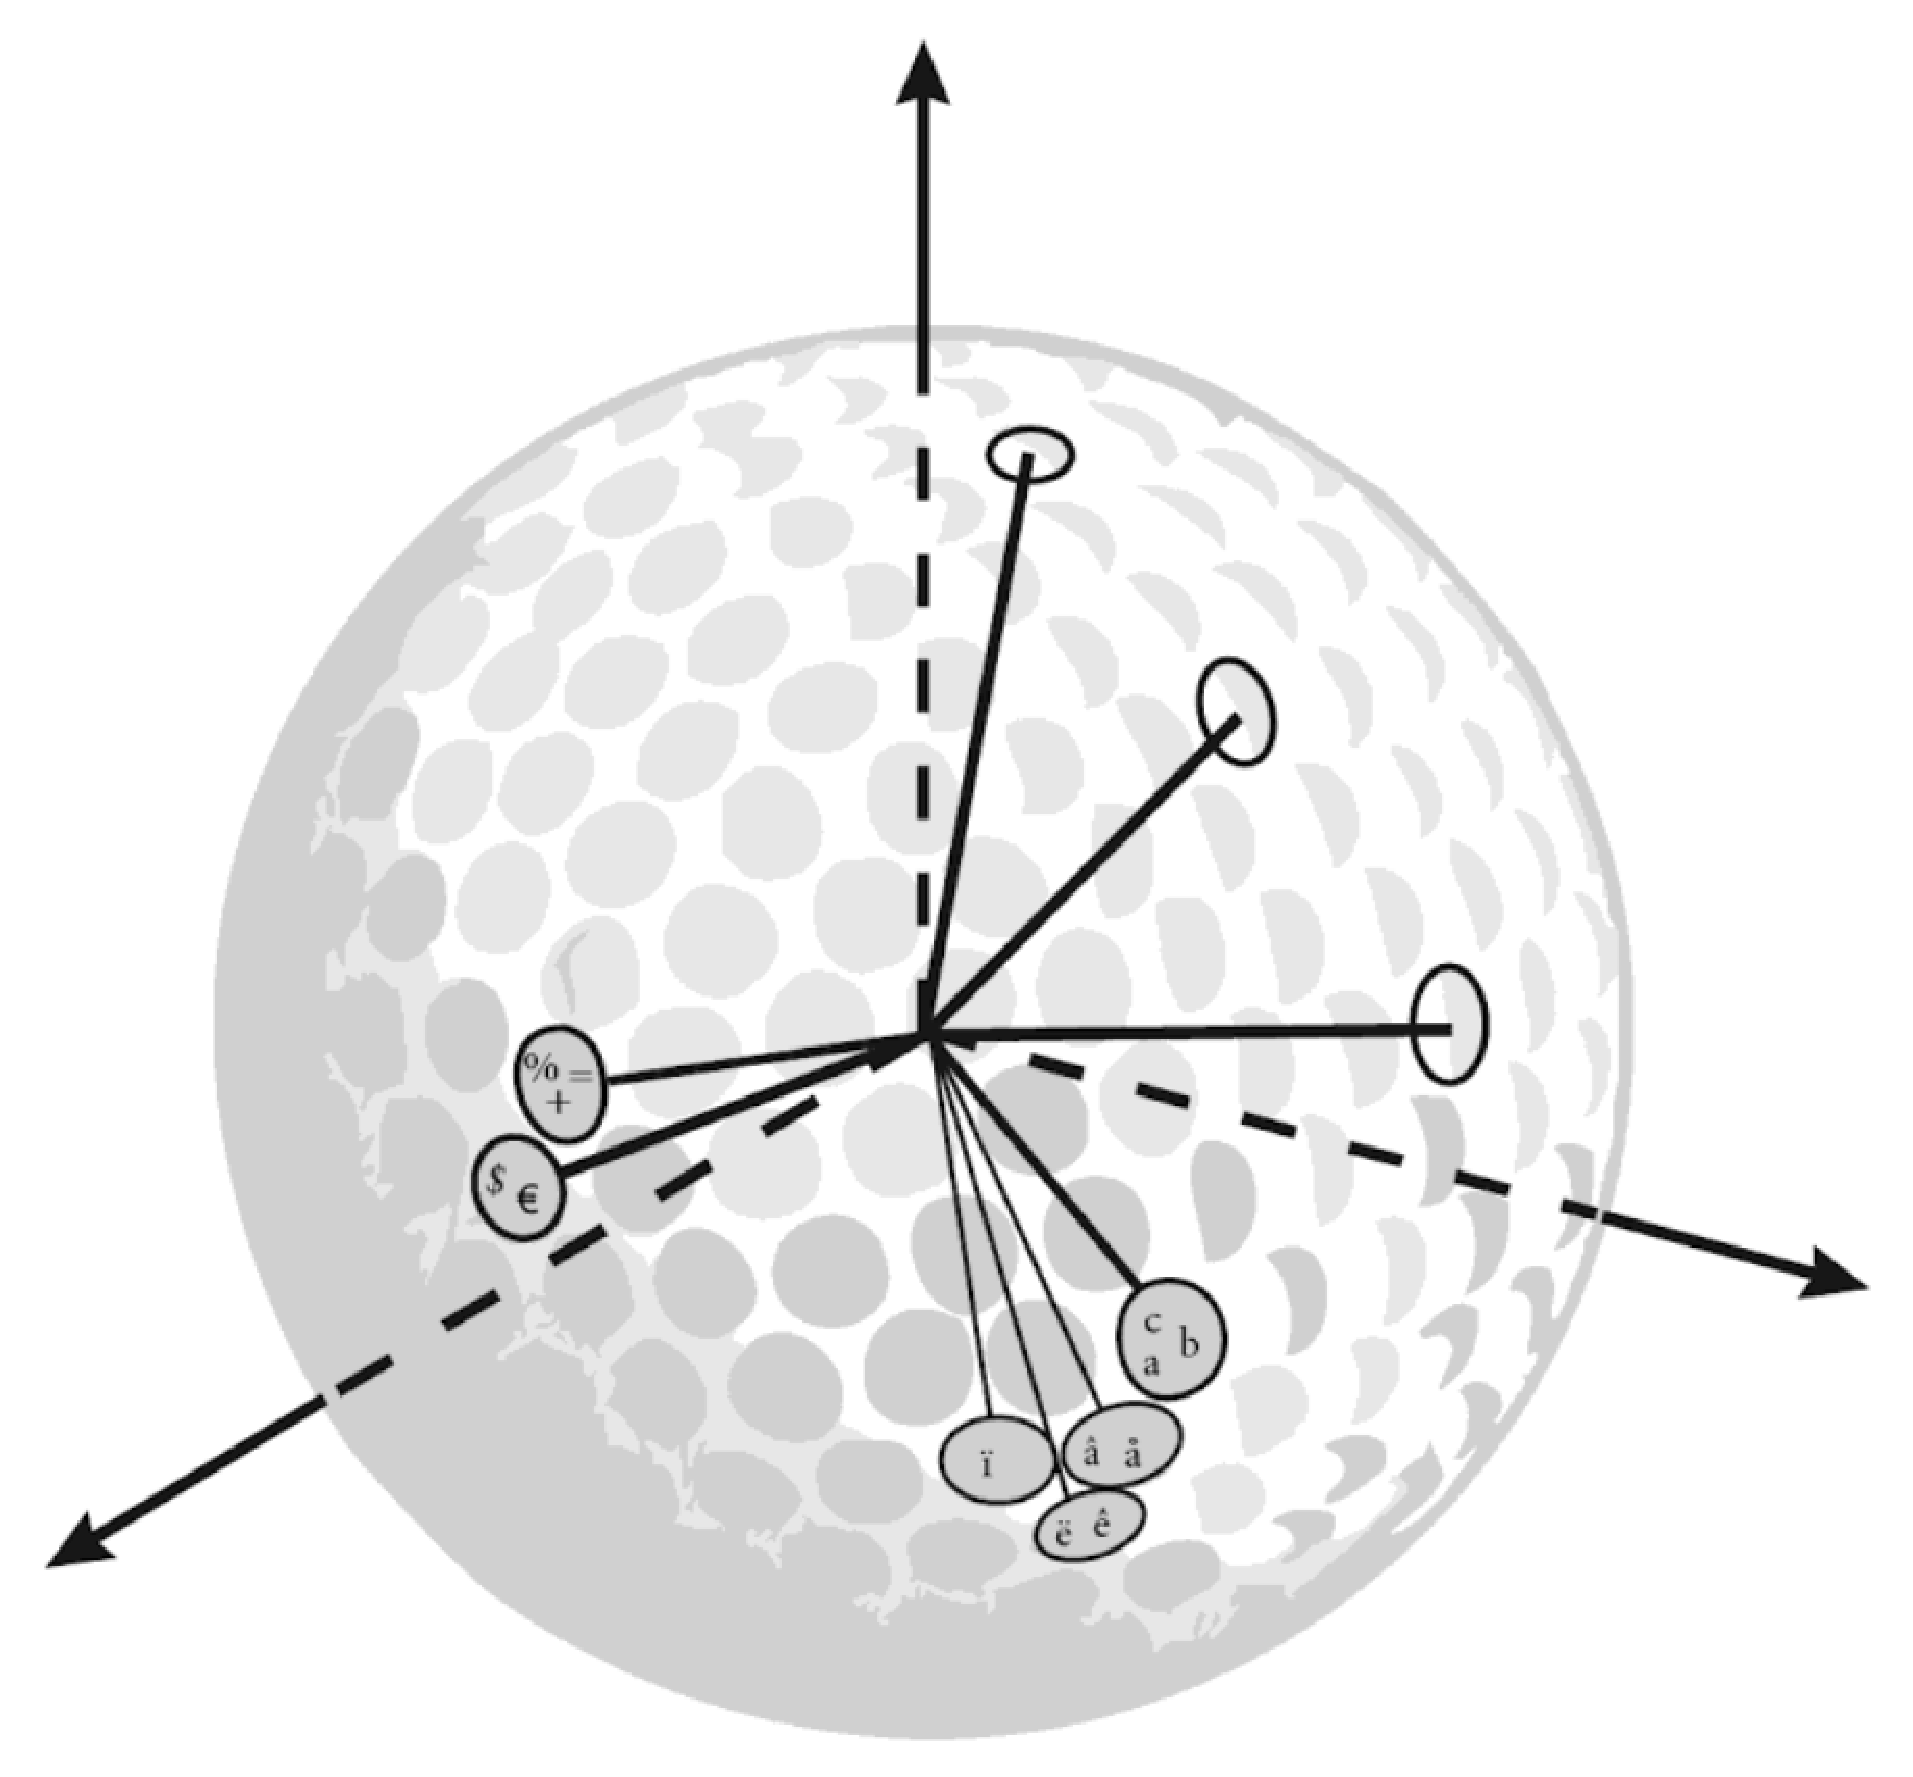
\includegraphics[width=0.55\textwidth]{imgs/conceptual_golfball.eps}
	\caption{"Conceptual golfball" depicting the idea of semantic vectors. Image source \cite{Eliasmith2013}.}
	\label{fig:conceptual_golfbal}
\end{figure}
Let $\vartheta \subset \mathcal{S}(D)$ be a vocabulary in the $D$-dimensional \ac{SPA}, where each vector $v \in \vartheta$ represents one item (i.e. a symbol, word or concept) in the representional space.
The content and size, i.e. the items of interest to be represented in such a vocabulary and their number as well as the way the representing vectors are established is highly task-dependent.
In its simplest form, all vectors in the vocabulary are chosen at random.
This approach is feasible due to the properties of high-dimensional vector spaces (cf. Theorem \ref{theorem:VSA_cossim_distribution} in Sec. \ref{sec:math_prop_vsas}) that the probability of randomly chosen vectors being dissimilar grows with vector dimension.
Therefore,  we have low probability of unintentionally confusing two different concept vectors.
However, this approach does not capture any similarities between items being represented.
Ideally, the goal is that the similarity between vectors in the vocabulary $\vartheta$ somewhat reflects the similarity between represented items.
Figure \ref{fig:conceptual_golfbal} depicts this idea: one subset of the space is assigned to vectors representing letters whereas another subset contains vectors representing special characters.
For a small number of items, the simplest way to create a vocabulary respecting some kind of similarity is to manually engineer the desired properties from randomly chosen vectors. 
Let us assume we want to derive representative vectors for five different classes of traffic participants, namely \emph{pedestrian}, \emph{bicycle}, \emph{motorcycle},  and \emph{car}.
A simple structured vocabulary could be constructed in the following way
\begin{align*}
\mathbf{PEDESTRIAN} &:= \mathbf{DRIVE} \varoast \mathbf{MUSCLE} + \mathbf{ACTUATOR} \varoast \mathbf{LEG} \varoast \mathbf{TWO} \\ 
\mathbf{BICYCLE} &:= \mathbf{DRIVE} \varoast \mathbf{MUSCLE} + \mathbf{ACTUATOR} \varoast \mathbf{WHEEL} \varoast \mathbf{TWO}\\
\mathbf{MOTORCYCLE} &:= \mathbf{DRIVE} \varoast \mathbf{MOTOR} + \mathbf{ACTUATOR} \varoast \mathbf{WHEEL} \varoast \mathbf{TWO}\\
\mathbf{CAR} &:= \mathbf{DRIVE} \varoast \mathbf{MOTOR} + \mathbf{ACTUATOR} \varoast \mathbf{WHEEL} \varoast \mathbf{FOUR},
\end{align*}
with all atomic vectors on the right side of the equations being chosen at random from $\mathcal{S}(D)$.\\
A more sophisticated way to create a vector vocabulary is to learn it automatically from data.
In contrast to purely random vocabularies, the idea here is that the learning system is able to capture the intrinsic similarity between objects in the vector representation.
Again, the choice of this learning paradigm (supervised vs. unsupervised) and architecture (e.g. \acp{CNN} or \acp{SOM}) depends not only on the given task, but also on the kind of similarity the vectors should encapsulate.
This can be visual similarity (e.g. items or objects that "look" similar), auditory similarity (e.g. objects producing similar sound), semantic similarity (e.g. words with similar meaning) or similarity in characteristics (e.g. similar motion characteristics).

A typical way of learning a vocabulary whose vectors conserve visual similarity in supervised fashion are \acp{CNN}.
These network architectures are inspired by the human visual cortex and compress high-dimensional visual input to lower dimensional representations.
They usually consist of a series of convolutional and pooling layers followed by one or more fully connected layers, where the last layer provides the classification result (cf. fig. \ref{fig:CNN_arch}).
The activity of the second-to-last layer (the last fully-connected one before the actual classification) for each known class in the data set can be considered a representational vector for the current visual input.
A simple way of getting a representative vector for each class is simply calculating the element-wise, normalized mean over all examples in the test set.
\todo{add reference to later chapter with traffic sign \ac{CNN}}
\begin{figure}[t]
	\centering
	\includegraphics[width=0.75\textwidth]{imgs/CNNArchitecture.jpg}
	\caption{\todo{Adapt image such that the second-to-last layer is highlighted}. Image adapted from \cite{Peemen2011}.}
	\label{fig:CNN_arch}
\end{figure}
A similar approach to derive vectors representing digits from $0$ to $9$ was used for the network performing the visual digit recognition task as part of the larger \ac{Spaun} model \cite{Eliasmith2012}, which was derived by training a \ac{DNN} consisting of four \ac{RBM} layers.
\todo{check this and reformulate}\\
The aforementioned approach to create vector vocabularies encapsulating visual similarity is 
\subsection{Encoding structure}
\subsection{Implementation in \acp{SNN}}

\todo{explain how modelling with VSAs works referring to neural modelling section and explain implementation in SNNs}\\
\todo{use conceptual golfball metaphor here}
\section{Summary}

